\RequirePackage{fix-cm}

\documentclass[12pt,a4paper,titlepage,oneside]{article}

\usepackage[T1]{fontenc}
\usepackage[utf8]{inputenc}
\usepackage[singlespacing]{setspace}
\usepackage{microtype}
\usepackage{indentfirst}
\usepackage[title]{appendix}
\usepackage{xurl}
\usepackage{enumerate}
\usepackage{amsmath,amssymb}
\usepackage[amsmath,amsthm,thmmarks]{ntheorem}
\usepackage{mathtools}
\usepackage{bm}
\usepackage{braket}
\usepackage{graphicx}
\usepackage{makecell}
\usepackage[justification=centering]{caption}
\usepackage{subcaption}
\usepackage{textcomp}
\usepackage{xcolor}
\usepackage{listings}
\usepackage{mcode}
\usepackage{chngcntr}
\usepackage{fancyhdr}
\usepackage[unicode]{hyperref}

\renewcommand{\contentsname}{Sadržaj}
\renewcommand{\abstractname}{Rezime}
\renewcommand{\figurename}{Slika}
\renewcommand{\tablename}{Tabela}
\renewcommand{\indexname}{Indeks pojmova}
\renewcommand{\refname}{Literatura}

\numberwithin{equation}{section}
\numberwithin{figure}{section}
\numberwithin{table}{section}

\renewcommand{\appendixname}{Dodatak}
\renewcommand{\appendixpagename}{Dodaci}

\newtheorem{thm}{Teorema}[section]
\newtheorem{stav}[thm]{Stav}
\newtheorem{lem}[thm]{Lema}
\newtheorem{posl}[thm]{Posledica}

\theoremstyle{definition}
\newtheorem{defi}{Definicija}[section]
\newtheorem{pri}{Primer}[section]
\newtheorem{zad}[pri]{Zadatak}

\theoremstyle{remark}
\newtheorem*{nap}{Napomena}

\renewcommand*{\proofname}{\textit{Dokaz}}

\DeclareMathOperator*{\argmin}{argmin}
\DeclarePairedDelimiterX{\norm}[1]{\lVert}{\rVert}{#1}
\DeclarePairedDelimiterX{\ip}[2]{\langle}{\rangle}{#1\mathrel{\delimsize|}#2}

\captionsetup[table]{aboveskip=8.5pt,belowskip=-13pt}

\lstset{
	numbers=left,
	numberstyle={\fontfamily{pcr}\selectfont},
	numbersep=22pt,
	breaklines=true,
	breakatwhitespace=true,
	breakindent=14.4pt,
	captionpos=b,
	abovecaptionskip=10pt,
	belowcaptionskip=10pt,
}

\renewcommand{\lstlistingname}{Algoritam}
\renewcommand{\lstlistlistingname}{Algoritmi}

\pagestyle{fancy}
\lhead{\leftmark}
\chead{}
\rhead{}
\lfoot{}
\cfoot{\thepage}
\rfoot{}

\title{Efikasnost avio kompanije u popunjavanju dostupnih sedišta}
\author{Andrija Stamenković, Jovana Savić}
\date{Septembar 2023.}

\makeatletter
\hypersetup
{
	pdftitle={\@title},
	pdfauthor={\@author},
	hidelinks=true,
	pdfstartview=FitH,
}
\makeatother

\begin{document}
\counterwithin{lstlisting}{section}
\pagenumbering{roman}

\makeatletter
\noindent
\begin{titlepage}
	\begin{center}
		
\includegraphics[width=0.187583508125\textwidth]{logo_uns_u_boji}
		\begin{minipage}[b]{0.60703298375\textwidth}
			\centering
			{\large \textsc{Univerzitet u Novom Sadu}}\\
			{\large \textsc{Prirodno-matematički fakultet}}\\
			{\large \textsc{Departman za matematiku}}\\
			{\large \textsc{i informatiku}}\\
			\vspace{10.5pt}
		\end{minipage}
		
\includegraphics[width=0.187583508125\textwidth]{pmf_ns}
	\end{center}
	
	\vfill
	
	\begin{flushleft}
		{\Large Andrija Stamenković\\Jovana Savić}
	\end{flushleft}
	
	\vfill
	
	\begin{center}
		{\huge \textbf{\@title}}
	\end{center}
		
	\begin{center}
		{\large - seminarski rad -}
	\end{center}
	
	\vfill
	
	\begin{flushright}
		{\large Mentor:}\\
		{\large dr Sanja Ružičić}
	\end{flushright}
	
	\vfill
	
	\begin{center}
		{\large Novi Sad, \@date}
	\end{center}
\end{titlepage}
\makeatother

\clearpage
\setcounter{page}{2}
\thispagestyle{empty}

\tableofcontents

\newpage
\pagenumbering{arabic}
\thispagestyle{empty}

\section{Uvod}\label{Uvod}

\setcounter{footnote}{0}

Posmatraju se podaci o operacijama i učinku jedne avio kompanije.\ Oni se odnose na:
\begin{enumerate}[1.]
	\item broj letova,
	
	\item broj sati letenja,
	
	\item broj pređenih kilometara u hiljadama,
	
	\item broj putnika,
	
	\item broj putničkih kilometara u hiljadama,
	
	\item broj kilometara dostupnih sedišta (proizvod dostupnih sedišta u avionu i pređenog rastojanja) u hiljadama i
	
	\item procenat zauzetih sedišta od onih koja su bila dostupna u avionu.
\end{enumerate}

Podaci su dati po mesecima počevši od Aprila 2014.\ pa do Februara 2023.\ fiskalne godine koja počinje u Aprilu.\ Veličina uzorka je $n = 119$.

Gornjih sedam promenljivih su prikazane stubastim grafikonima na Slikama \ref{bar1}\,-\,\ref{bar7}, gde su njihove vrednosti date hronološki po mesecima.

\begin{figure}[h!]
	\centering
	\captionsetup{justification=centering}
	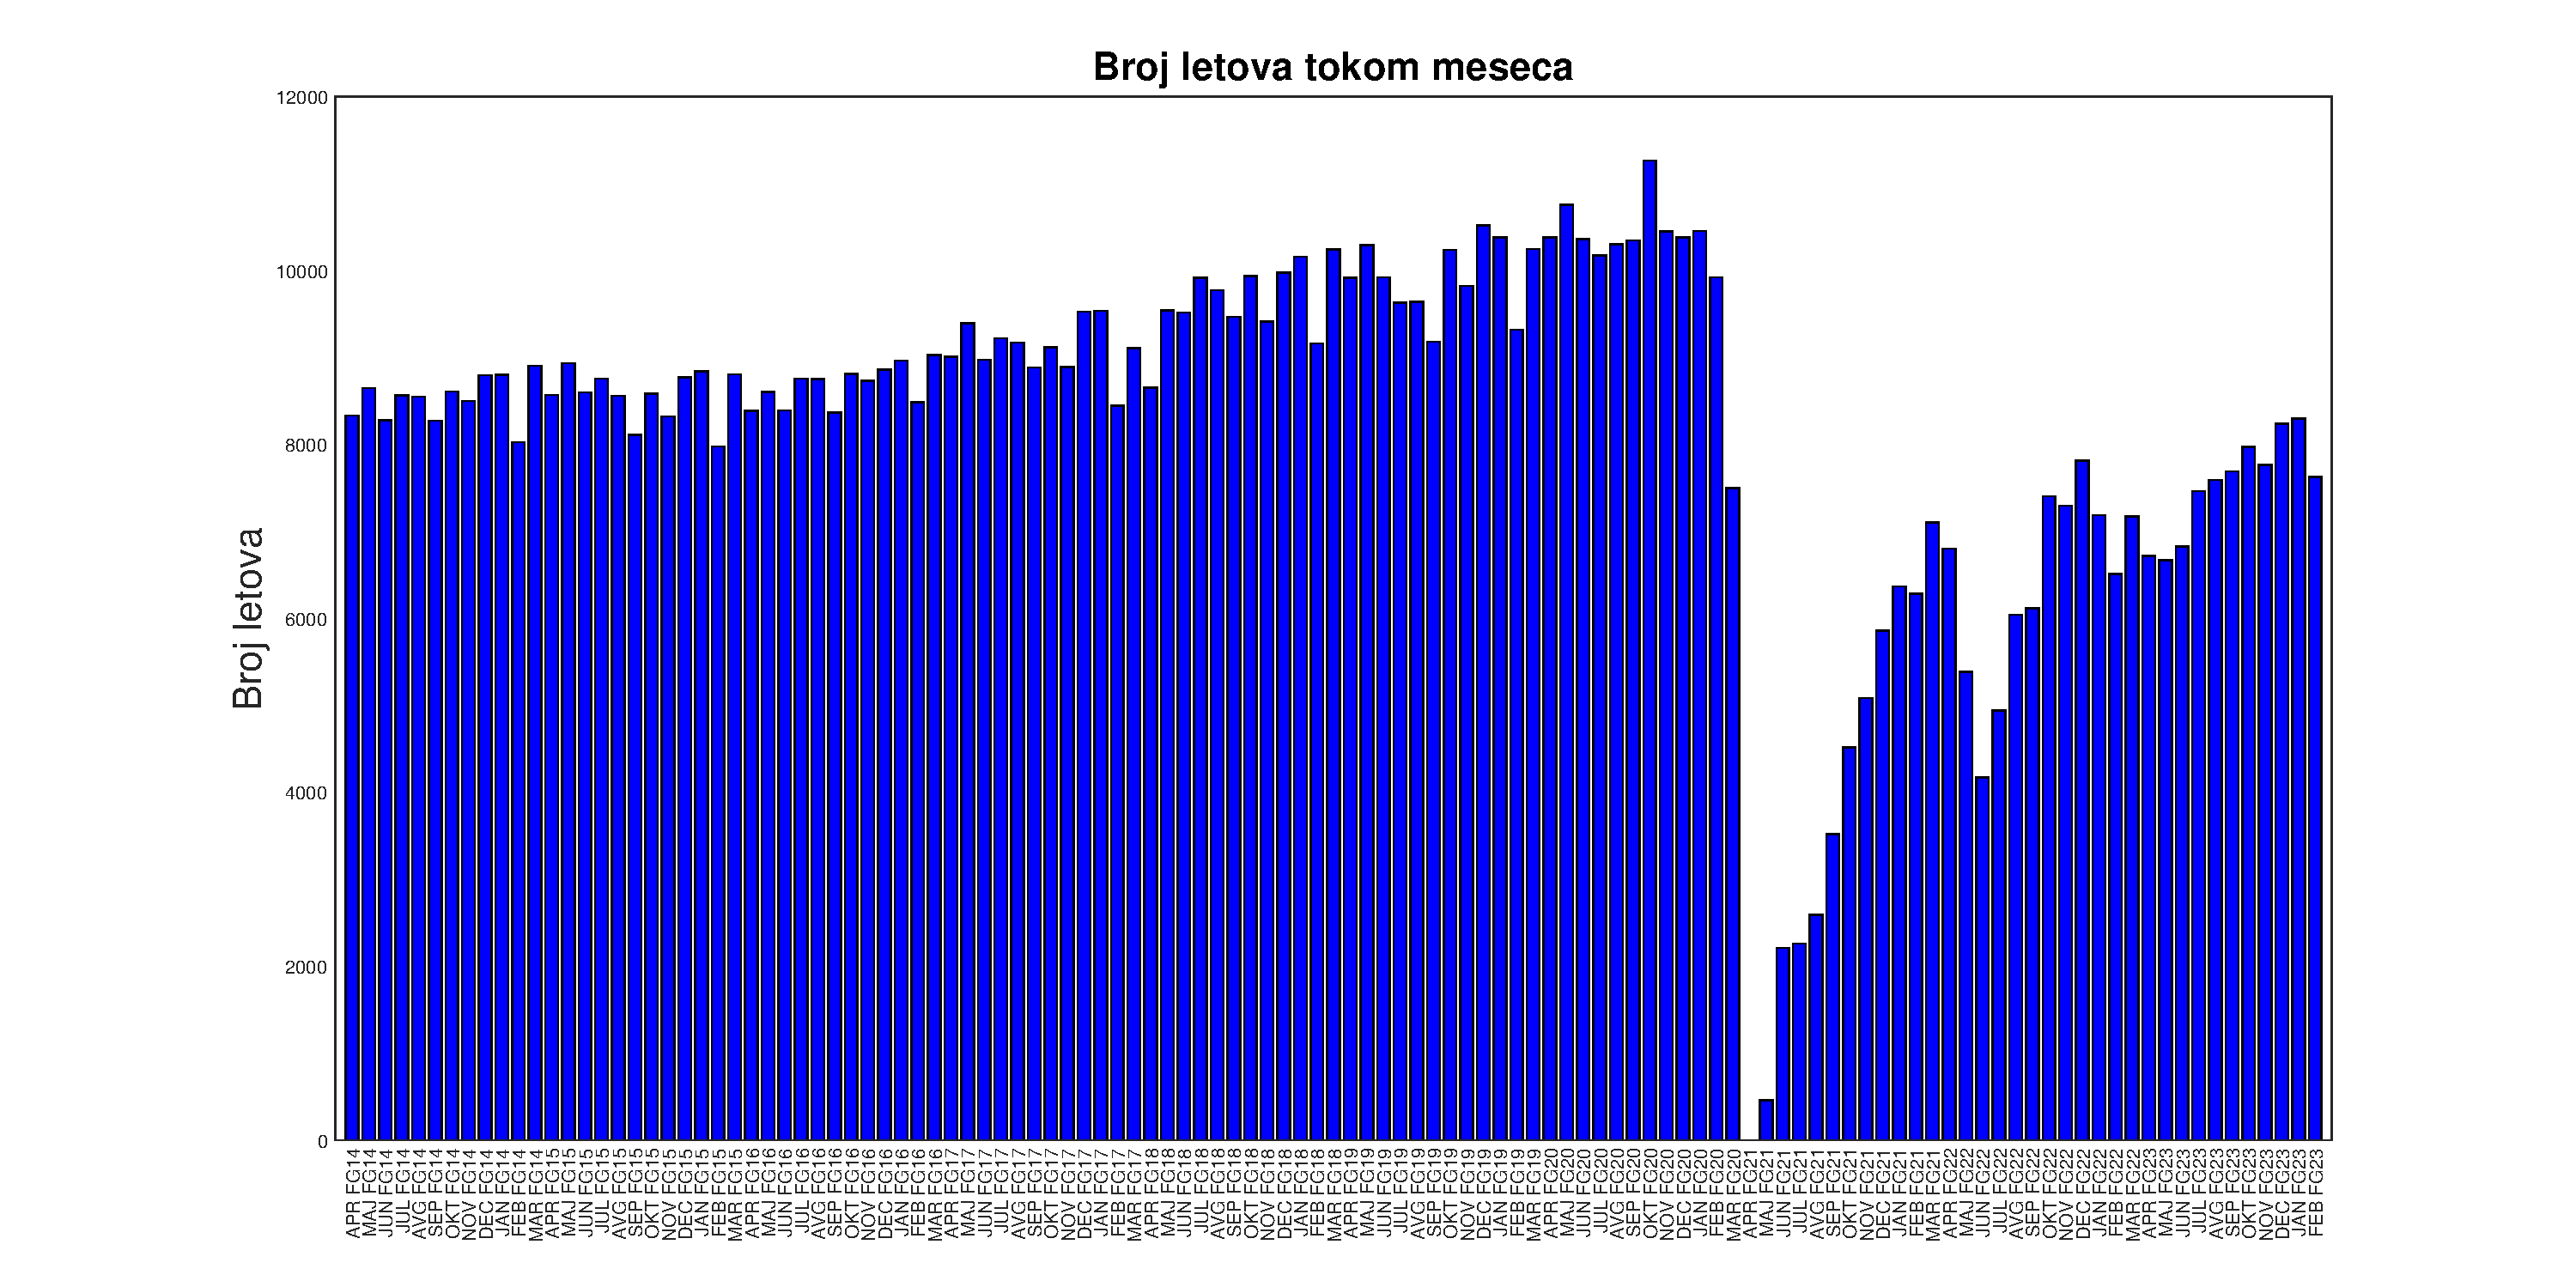
\includegraphics[width=0.98\textwidth]{bar1}
	\caption{Broj letova tokom meseca}
	\label{bar1}
\end{figure}

\begin{figure}[h!]
	\centering
	\captionsetup{justification=centering}
	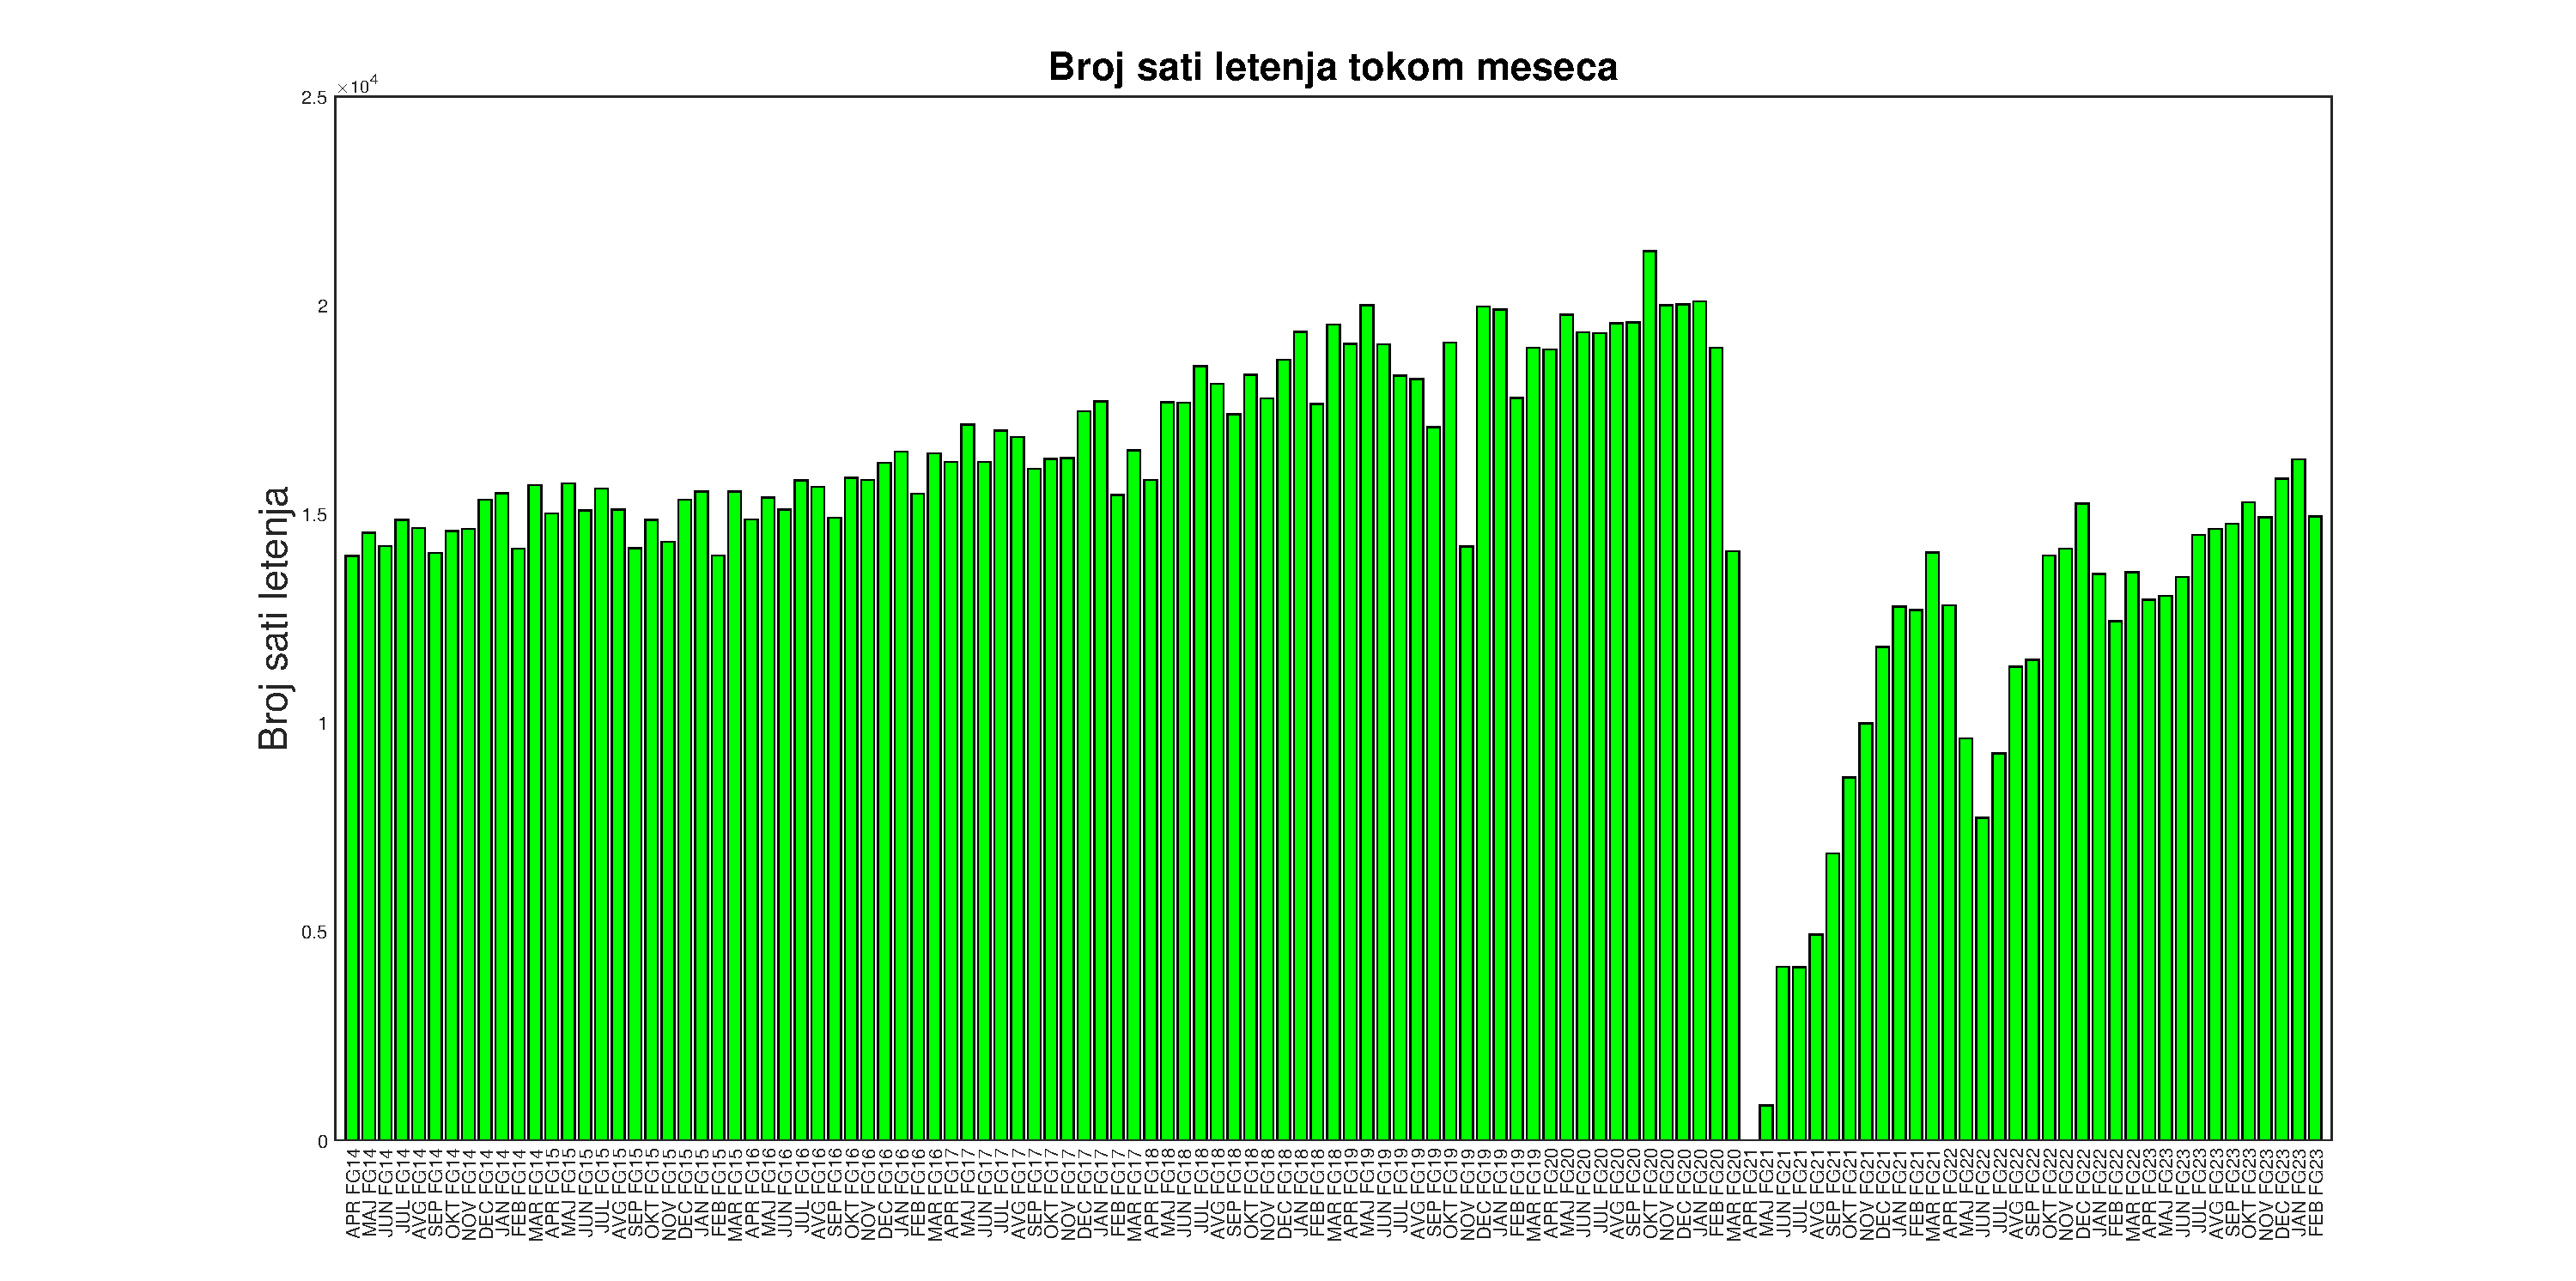
\includegraphics[width=0.98\textwidth]{bar2}
	\caption{Broj sati letenja tokom meseca}
\end{figure}

\begin{figure}[h!]
	\centering
	\captionsetup{justification=centering}
	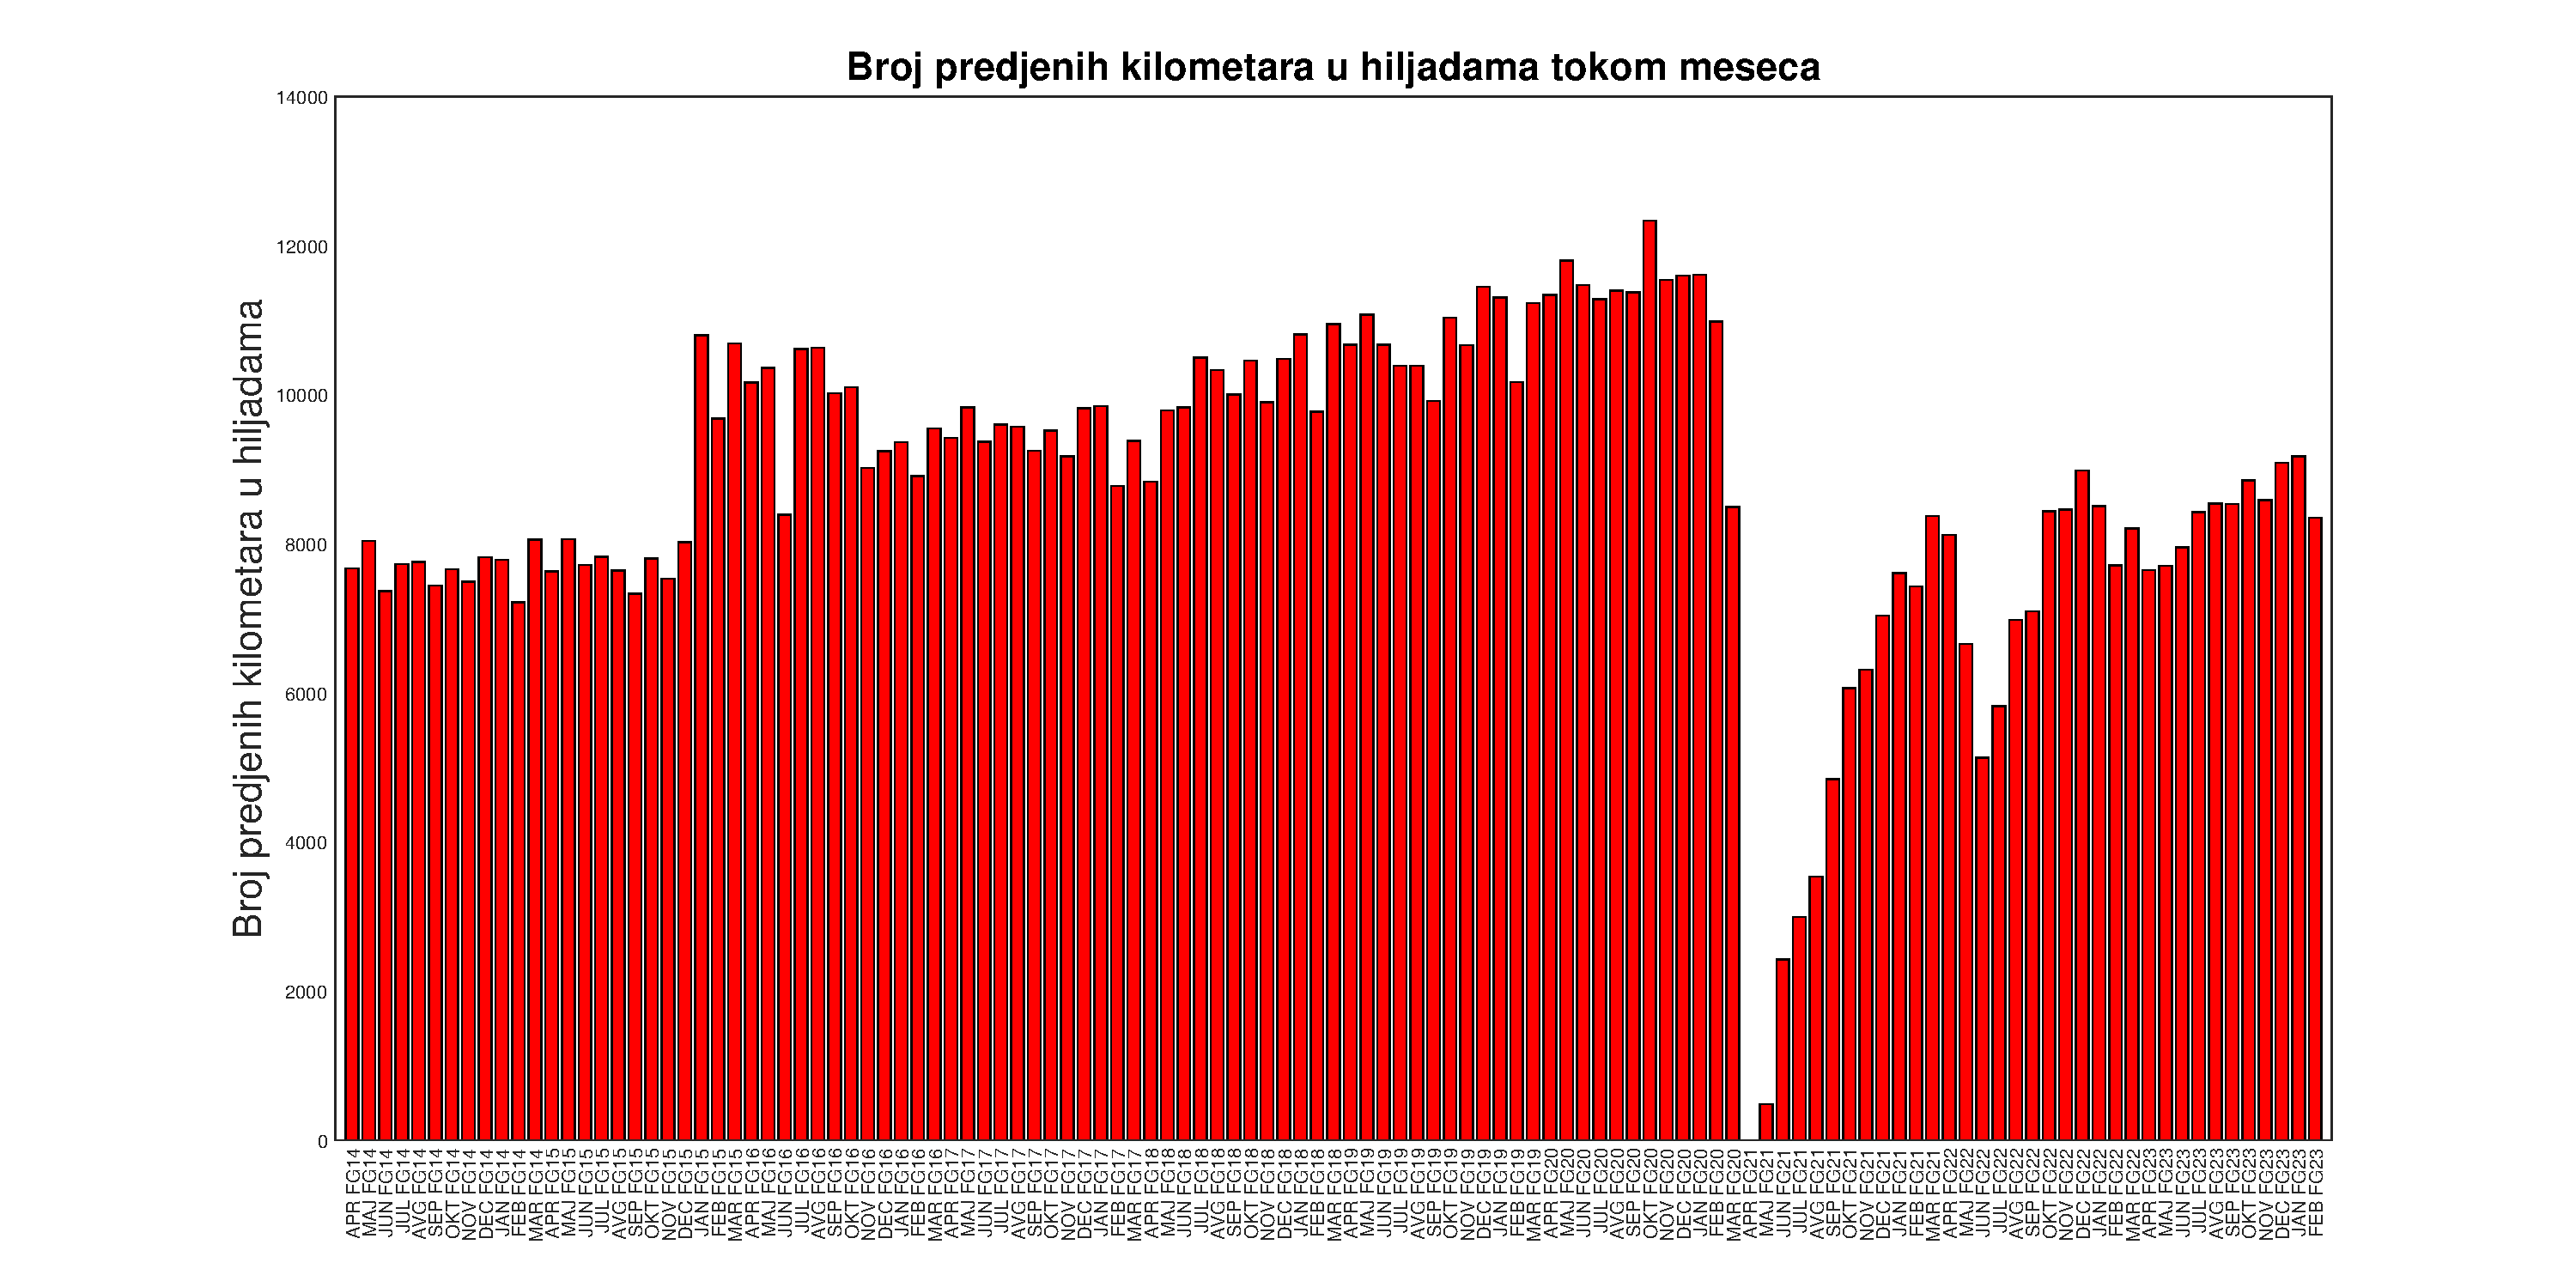
\includegraphics[width=0.98\textwidth]{bar3}
	\caption{Broj pređenih kilometara u hiljadama tokom meseca}
\end{figure}

\begin{figure}[h!]
	\centering
	\captionsetup{justification=centering}
	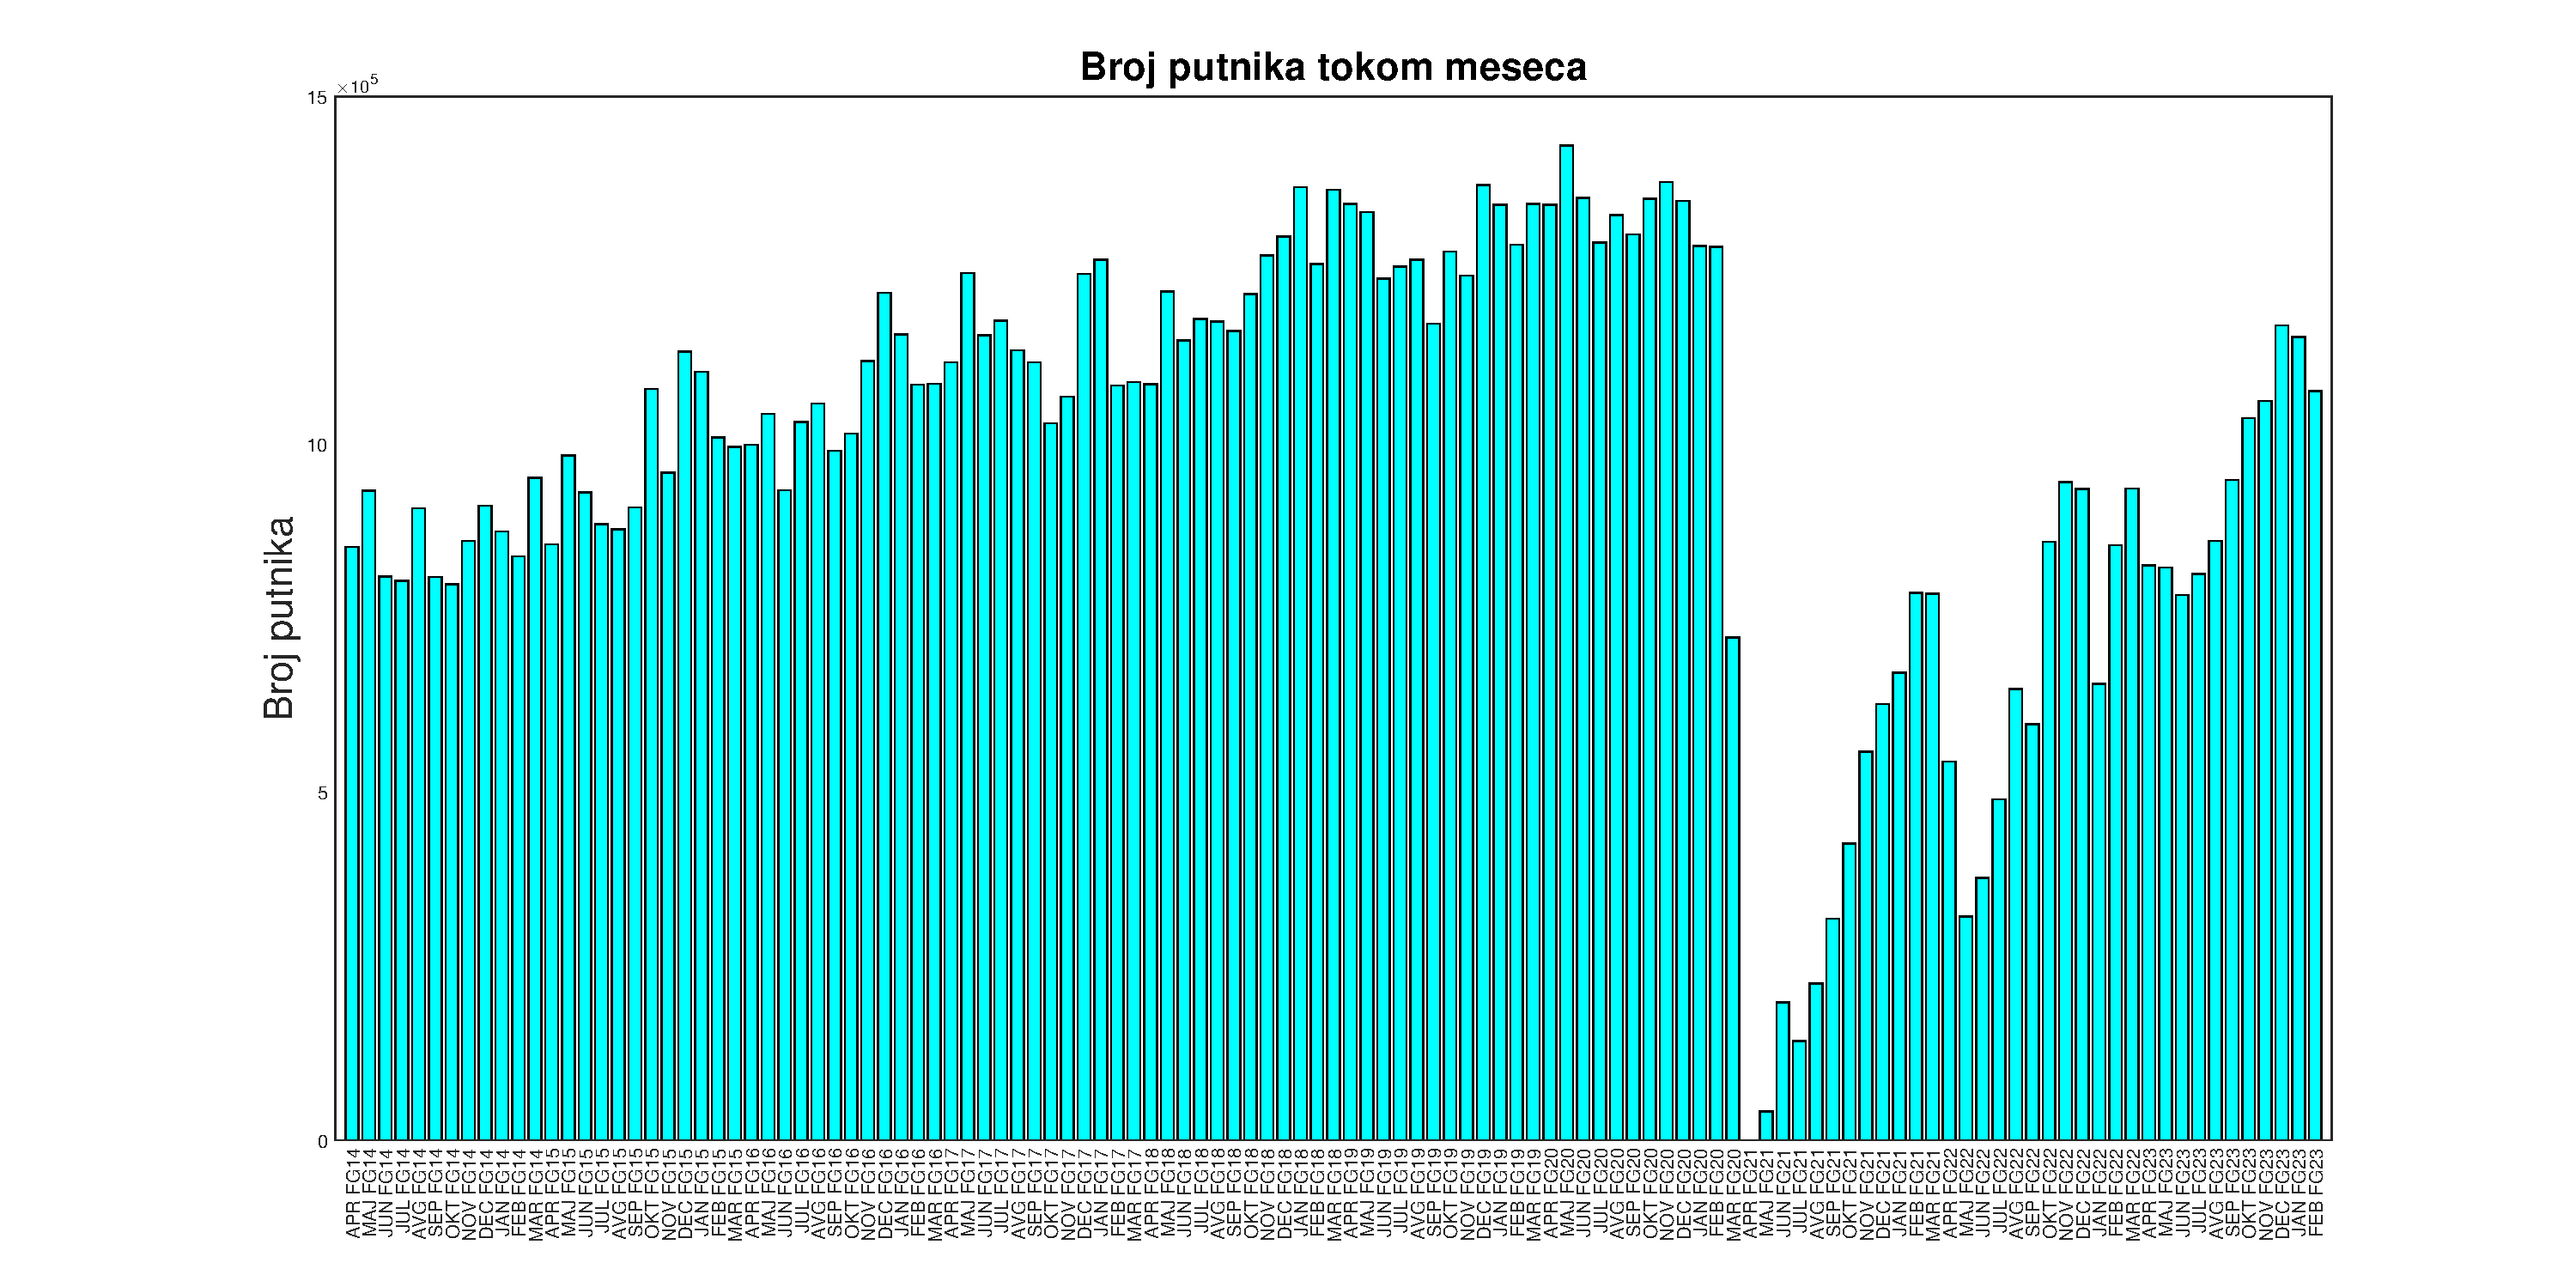
\includegraphics[width=0.98\textwidth]{bar4}
	\caption{Broj putnika tokom meseca}
\end{figure}

\begin{figure}[h!]
	\centering
	\captionsetup{justification=centering}
	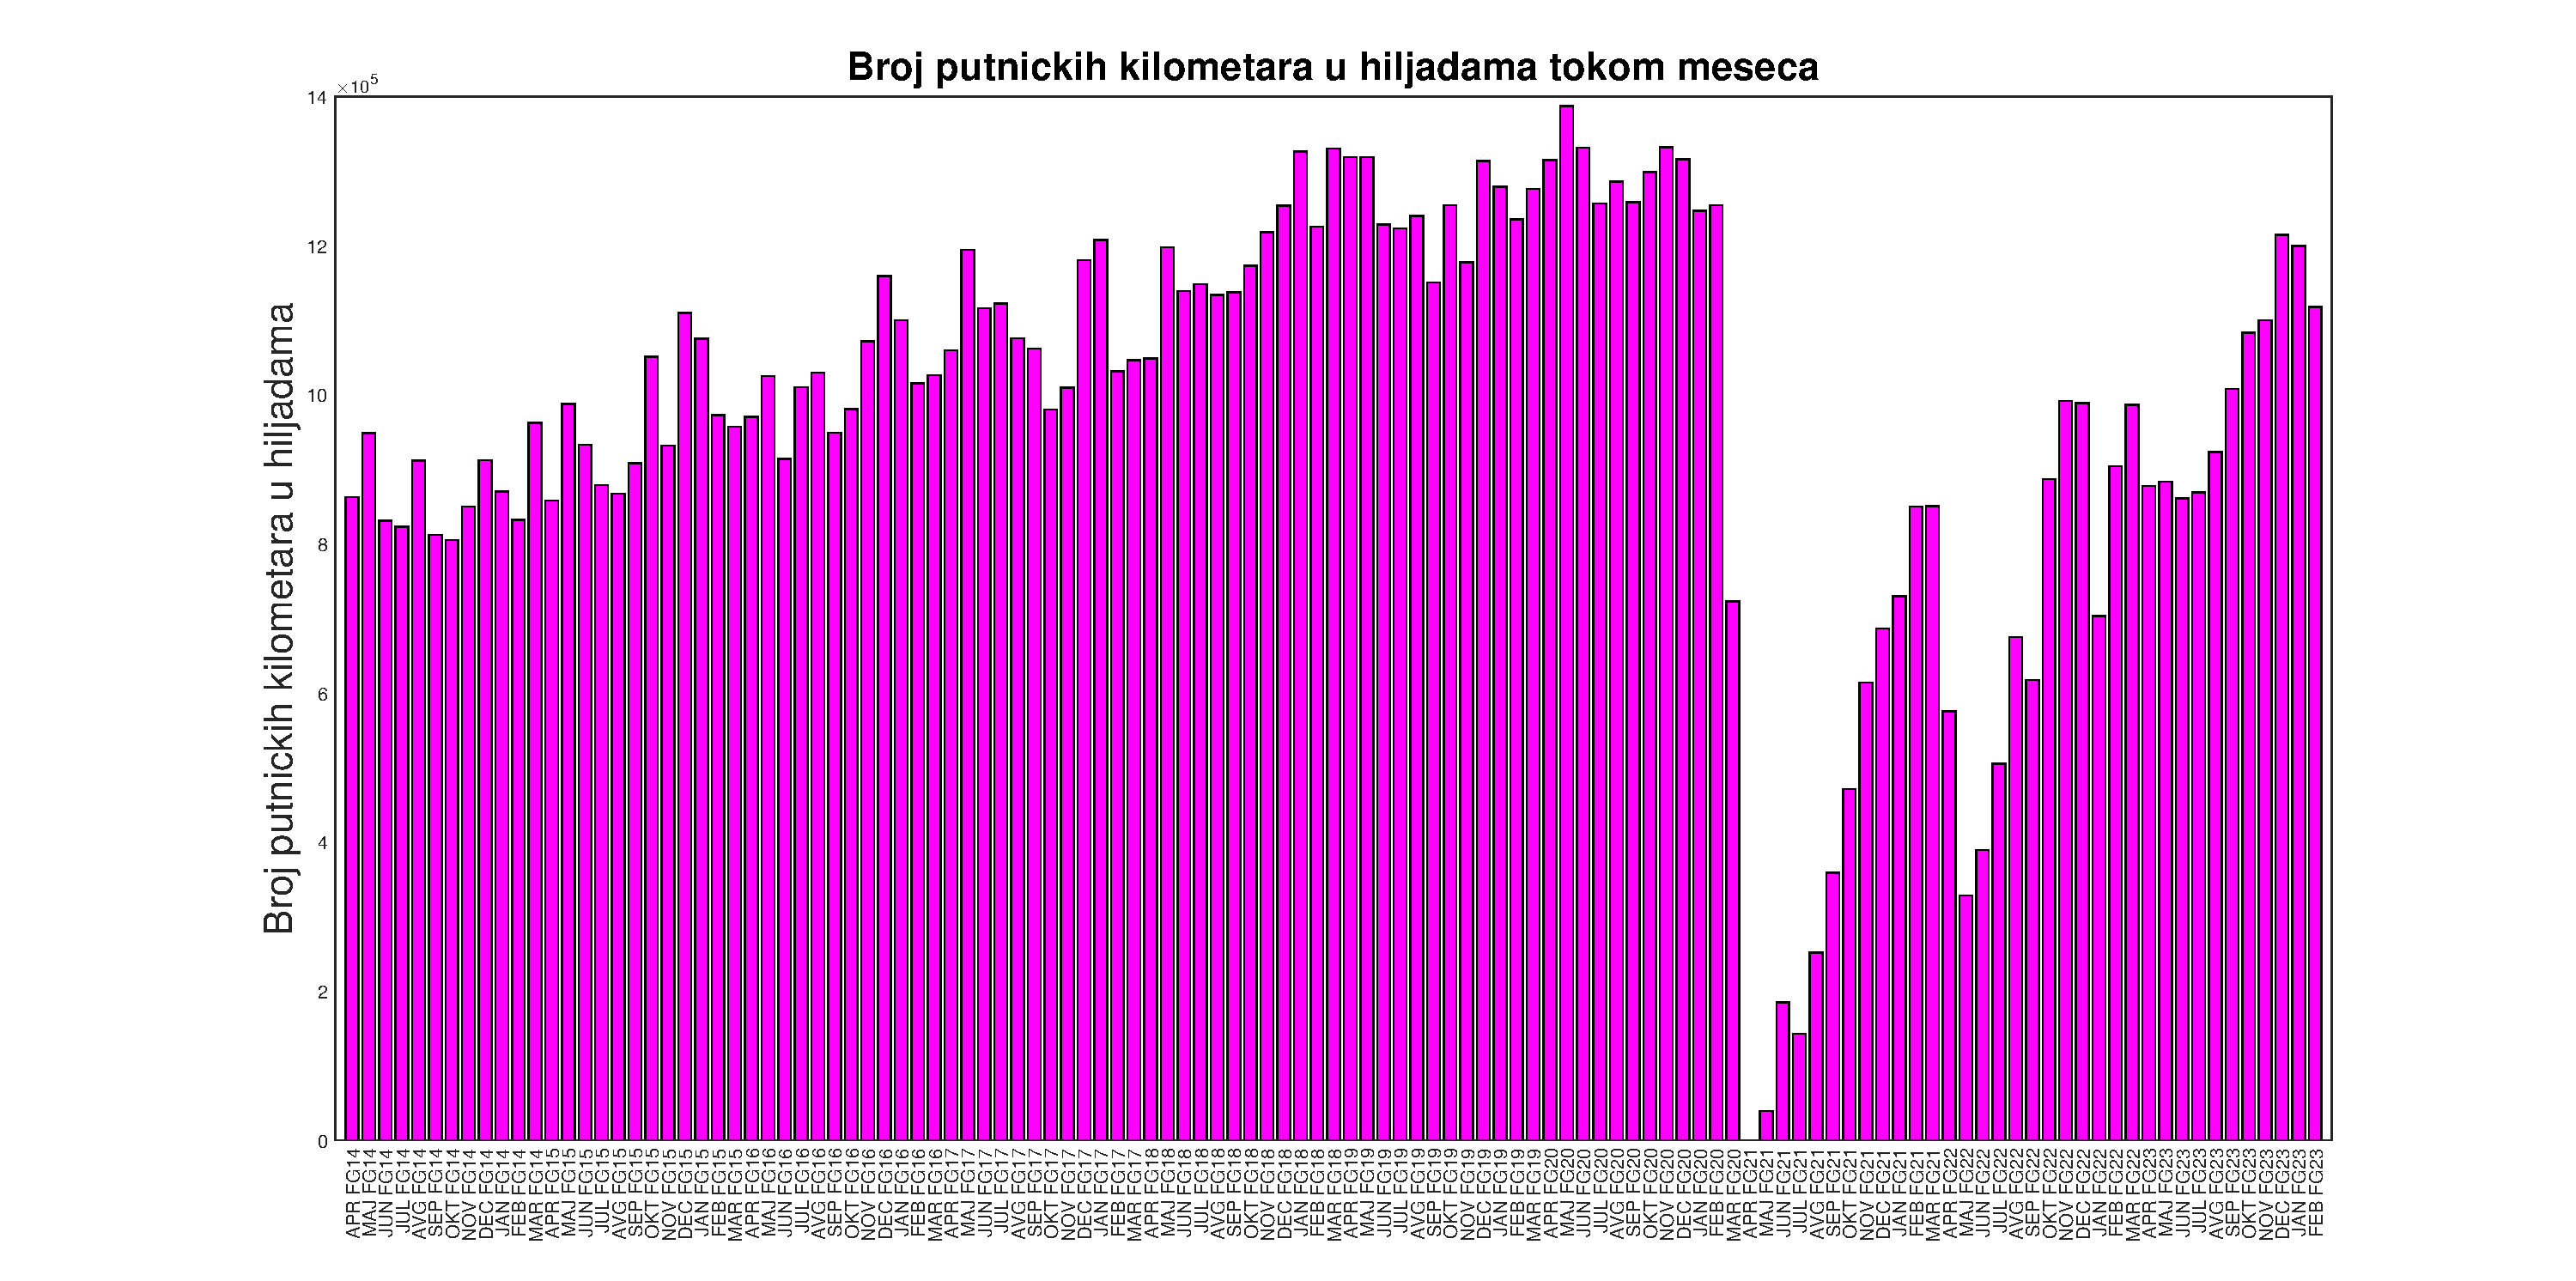
\includegraphics[width=0.98\textwidth]{bar5}
	\caption{Broj putničkih kilometara u hiljadama tokom meseca}
\end{figure}

\begin{figure}[h!]
	\centering
	\captionsetup{justification=centering}
	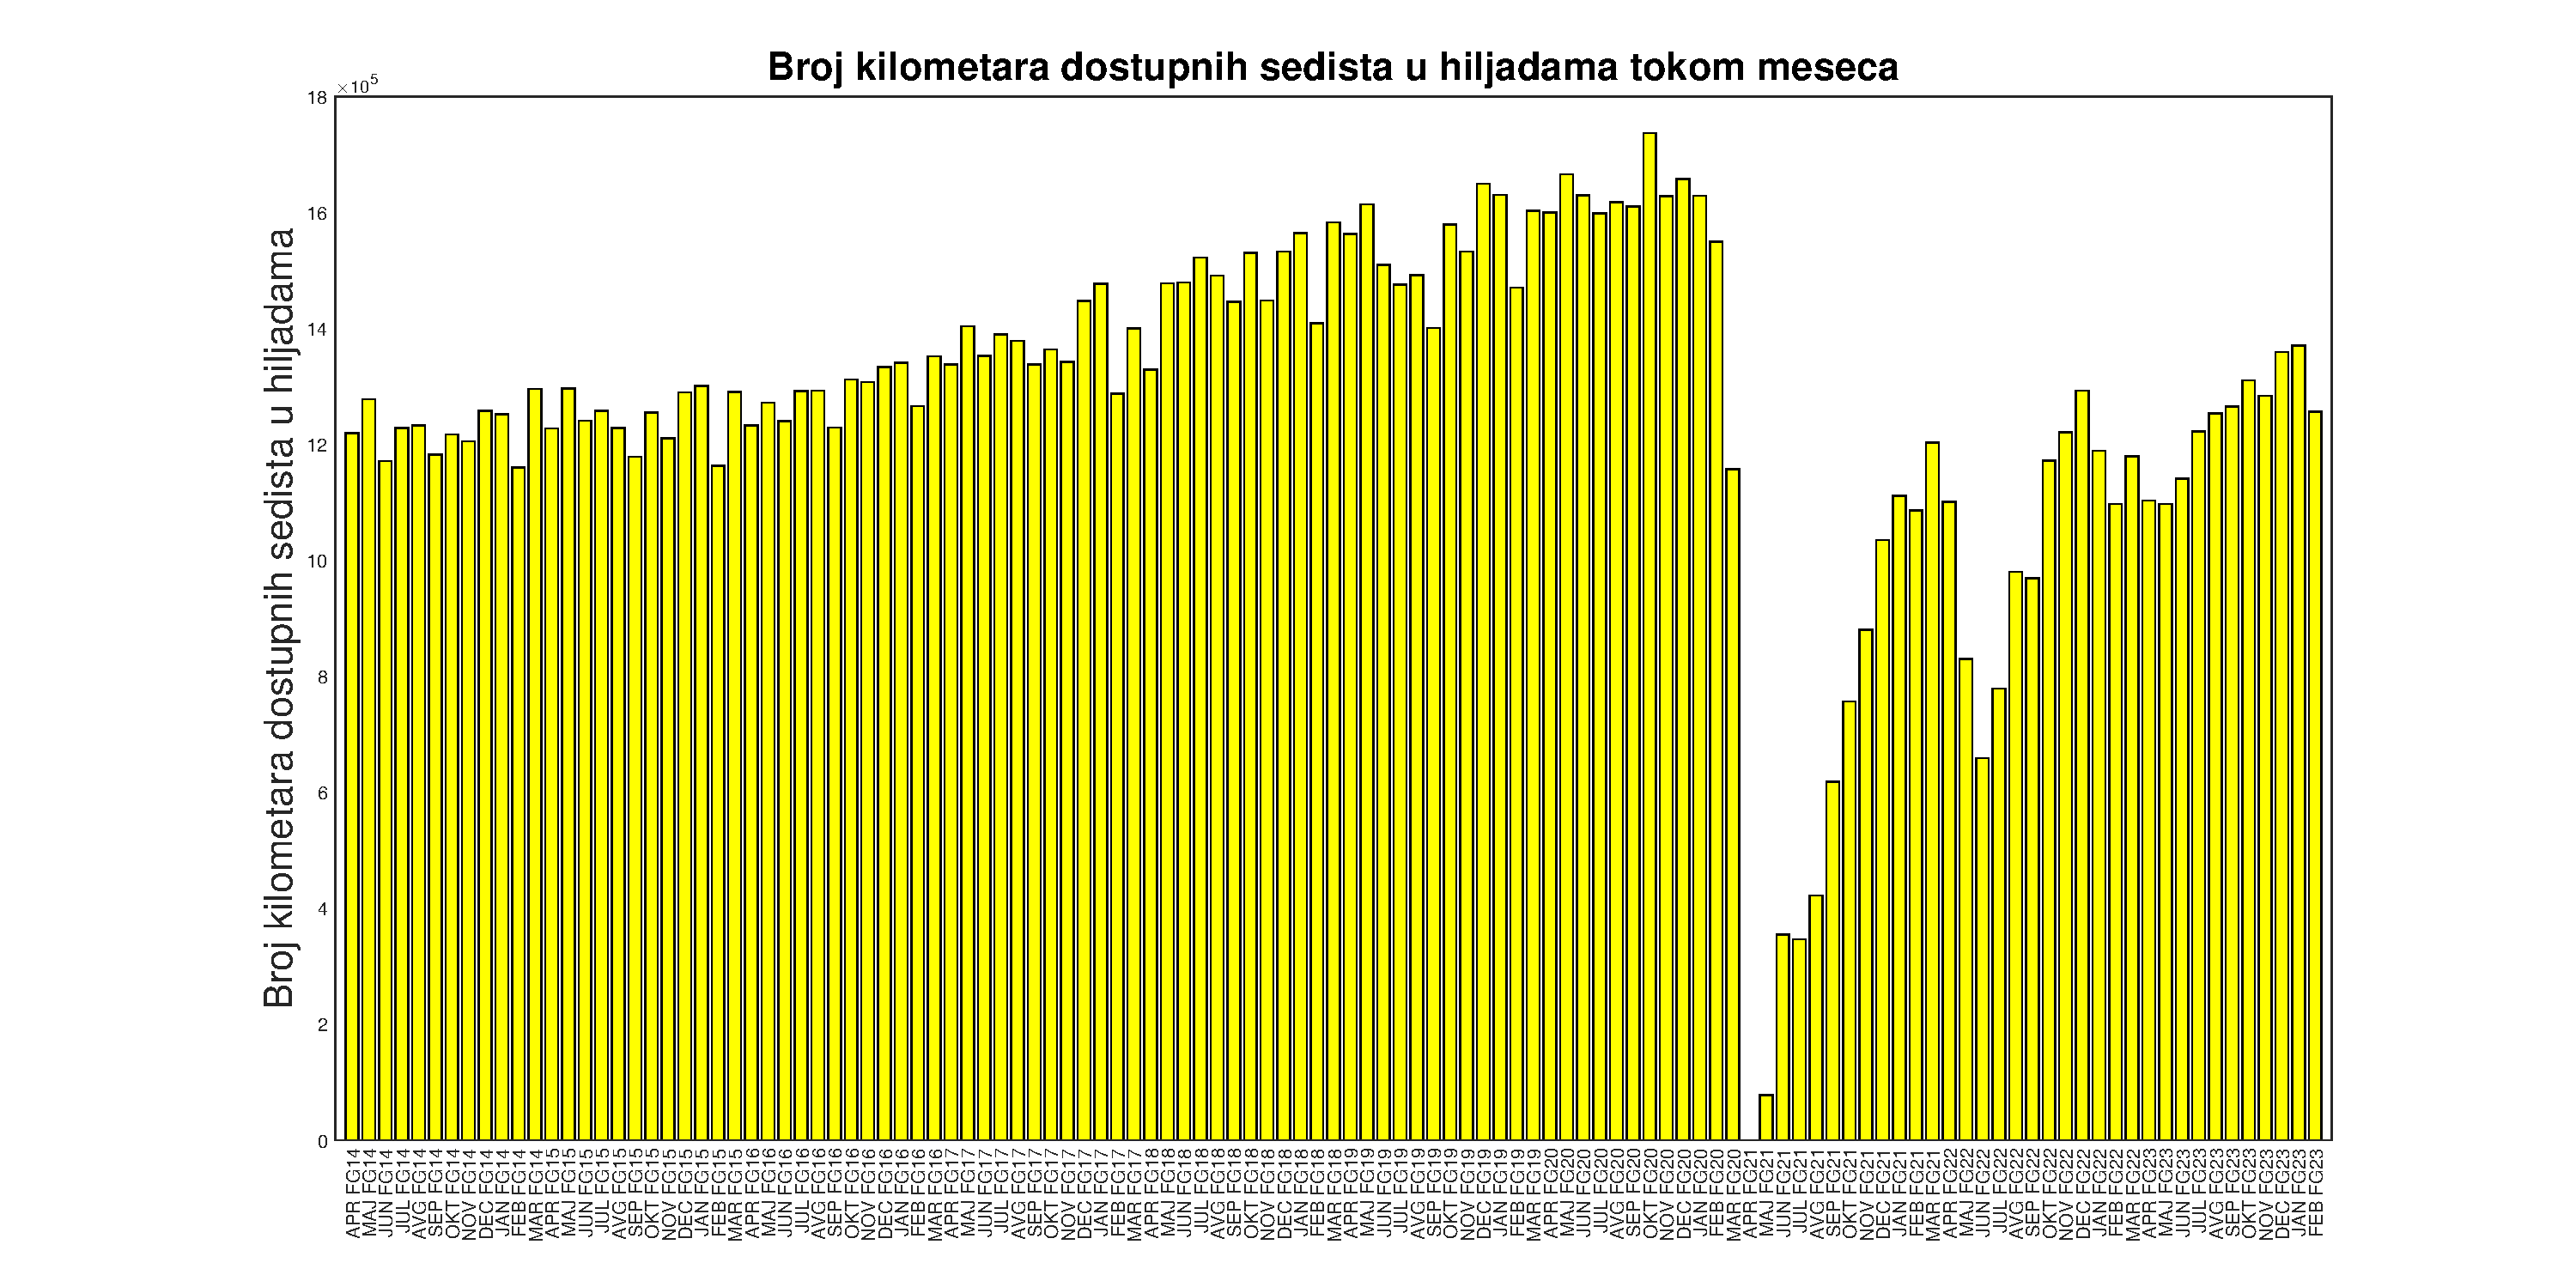
\includegraphics[width=0.98\textwidth]{bar6}
	\caption{Broj kilometara dostupnih sedišta u hiljadama tokom meseca}
\end{figure}

\begin{figure}[h!]
	\centering
	\captionsetup{justification=centering}
	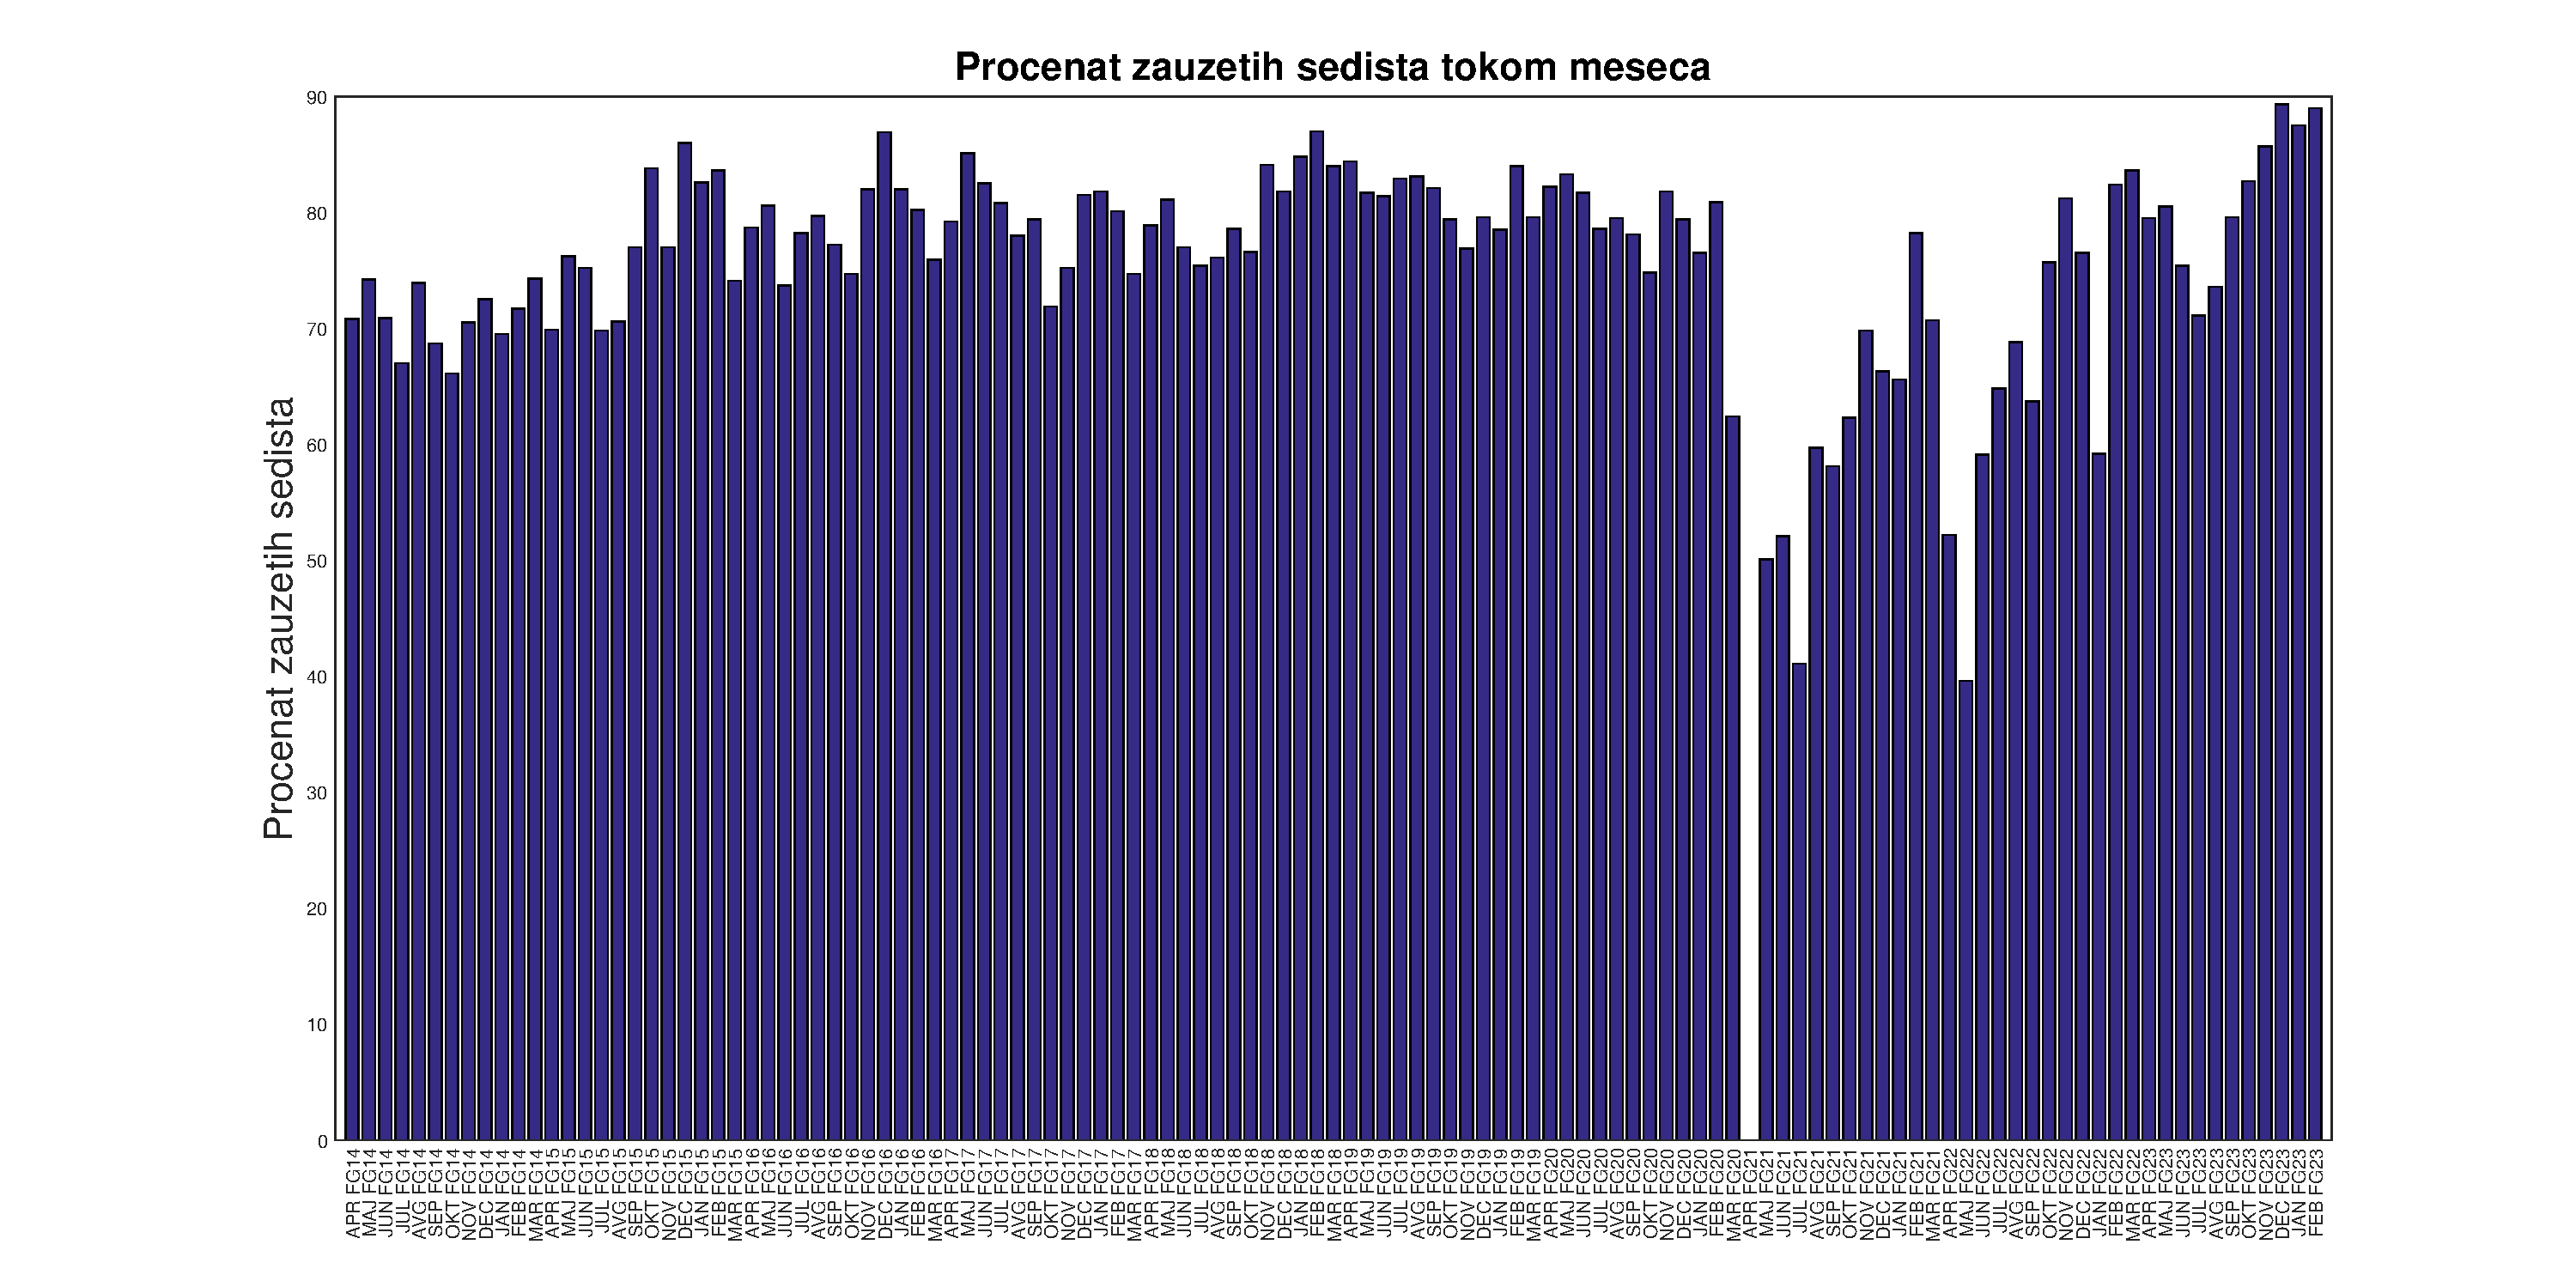
\includegraphics[width=0.98\textwidth]{bar7}
	\caption{Procenat zauzetih sedišta tokom meseca}
	\label{bar7}
\end{figure}

Aprila 2021.\ fiskalne godine je, zbog pandemije COVID-19, došlo do naglog pada svih datih promenljivih na nulu, nakon čega je došlo do oporavka.\ Prvih šest promenljivih su se u narednih skoro tri godine vratile na nivo manji od prethodnog.\ Jedini izuzetak je sedma promenljiva, procenat zauzetih sedišta, za koju su na kraju tog perioda zabeležene vrednosi veće od svih prethodnih.

Za date promenljive su nađeni srednja vrednost (aritmetička sredina), minimum, prvi kvartil, medijana (tj.\ drugi kvartil), treći kvartil, maksimum, moda sa njenom učestalošću pojavljivanja, popravljena varijansa (tj.\ disper-zija), popravljeno standardno odstupanje i međukvartilni opseg.\ Rezultati su, respektivno, dati na Slikama \ref{mean_arr}\,-\,\ref{iqr_arr} po kolonama, gde broj kolone odgovara rednom broju promenljive na listi sa početka ovog poglavlja.

\begin{figure}[h!]
	\centering
	\captionsetup{justification=centering}
	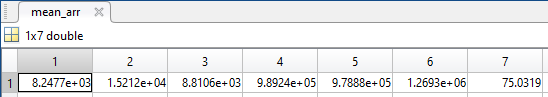
\includegraphics[width=0.68\textwidth]{mean_arr}
	\caption{Srednja vrednost (aritmetička sredina)}
	\label{mean_arr}
\end{figure}

\begin{figure}[h!]
	\centering
	\captionsetup{justification=centering}
	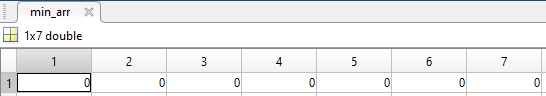
\includegraphics[width=0.68\textwidth]{min_arr}
	\caption{Minimum}
\end{figure}

\begin{figure}[h!]
	\centering
	\captionsetup{justification=centering}
	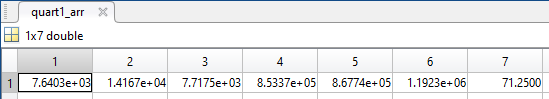
\includegraphics[width=0.68\textwidth]{quart1_arr}
	\caption{Prvi kvartil}
\end{figure}

\begin{figure}[h!]
	\centering
	\captionsetup{justification=centering}
	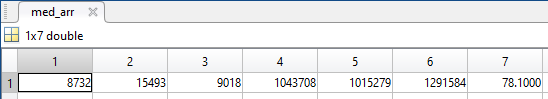
\includegraphics[width=0.68\textwidth]{med_arr}
	\caption{Medijana (tj.\ drugi kvartil)}
\end{figure}

\begin{figure}[h!]
	\centering
	\captionsetup{justification=centering}
	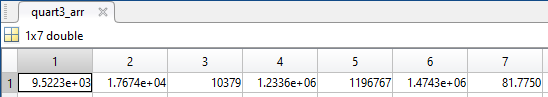
\includegraphics[width=0.68\textwidth]{quart3_arr}
	\caption{Treći kvartil}
\end{figure}

\begin{figure}[h!]
	\centering
	\captionsetup{justification=centering}
	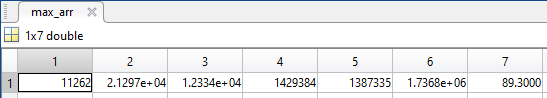
\includegraphics[width=0.68\textwidth]{max_arr}
	\caption{Maksimum}
\end{figure}

\begin{figure}[h!]
	\centering
	\captionsetup{justification=centering}
	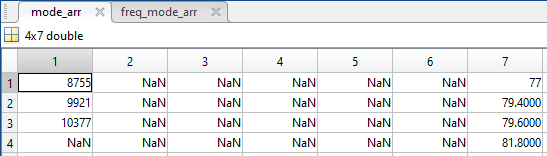
\includegraphics[width=0.68\textwidth]{mode_arr}
	\caption{Moda}
\end{figure}

\begin{figure}[h!]
	\centering
	\captionsetup{justification=centering}
	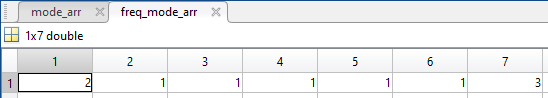
\includegraphics[width=0.68\textwidth]{freq_mode_arr}
	\caption{Učestalost pojavljivanja mode}
\end{figure}

\begin{figure}[h!]
	\centering
	\captionsetup{justification=centering}
	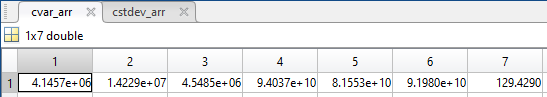
\includegraphics[width=0.68\textwidth]{cvar_arr}
	\caption{Popravljena varijansa (tj.\ disperzija)}
\end{figure}

\begin{figure}[h!]
	\centering
	\captionsetup{justification=centering}
	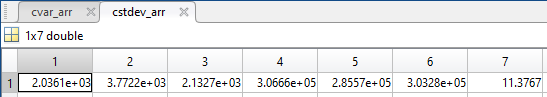
\includegraphics[width=0.68\textwidth]{cstdev_arr}
	\caption{Popravljeno standardno odstupanje}
\end{figure}

\begin{figure}[h!]
	\centering
	\captionsetup{justification=centering}
	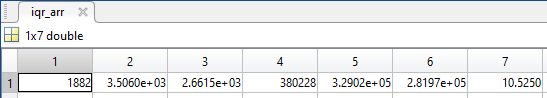
\includegraphics[width=0.68\textwidth]{iqr_arr}
	\caption{Međukvartilni opseg}
	\label{iqr_arr}
\end{figure}

Na primer, medijana četvrte promenljive, broj putnika, iznosi $1043708$. Što se tiče mode, promenljiva u kojoj se svaka vrednost javlja najviše jedanput nema modu, pa je povratna vrednost $\text{NaN}$ (od engleskog \textit{Not a Number}). Radi preglednosti, svi rezultati su prikazani u jednoj matrici dobijene pomoću (programerske) funkcije \texttt{nancat} koja vrši konkatenaciju matrica po željenoj dimenziji i na praznim mestima ispisuje $\text{NaN}$ (videti \hyperref[nancat]{Algoritam \ref*{nancat}}).\ Prema tome, sedma promenljiva, procenat zauzetih sedišta, je multimodalna, jer moda uzima vrednosti $77$, $79.4$, $79.6$ i $81.8$ po $3$ puta.

Dodatno, izračunati su uzorački koeficijenti korelacije.\ Rezultati su prika-zani na \hyperref[Rho]{Slici \ref*{Rho}}, gde broj kolone, odnosno vrste, odgovara rednom broju promenljive na listi.

\begin{figure}[h!]
	\centering
	\captionsetup{justification=centering}
	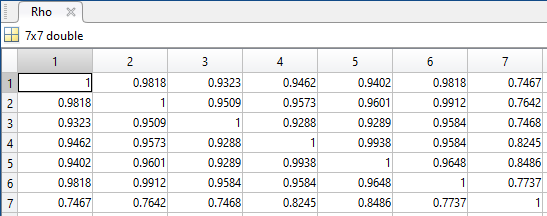
\includegraphics[width=0.68\textwidth]{Rho}
	\caption{Uzorački koeficijenti korelacije parova promenljivih}
	\label{Rho}
\end{figure}

Na primer, uzoračka korelacija između prve i četvrte promenljive, tj.\ broja letova i broja putnika, je $0.9462$.\ Kao što je poznato, korelacija promenljive sa samom sobom je $1$ i ona je simetrična, tj.\ redosled para promenljivih ne utiče na rezultat.\ Za sedmu promenljivu, tj.\ procenat zauzetih sedišta, uzorački koeficijenti korelacije uzimaju vrednosti između $0.74$ i $0.85$, dok su sve ostale vrednosti veće od $0.92$.

Urađen je još i Pirsonov hi-kvadrat test da bi se ispitalo da li date pro-menljive imaju normalnu raspodelu.\ Rezultati su prikazani na \hyperref[HP]{Slici \ref*{HP}}, gde broj kolone odgovara rednom broju promenljive na listi.\ U prvom redu je broj prihvaćene hipoteze, gde broj $0$ znači da je prihvaćena nulta hipoteza, tj.\ da posmatrana promenljiva ima normalnu raspodelu, dok broj $1$ znači da je prihvaćena alternativna hipoteza, tj.\ da posmatrana promenljiva nema normalnu raspodelu, na nivou značajnosti $0.05$.\ U drugom redu je odgovarajuća $p$-vrednost.

\begin{figure}[h!]
	\centering
	\captionsetup{justification=centering}
	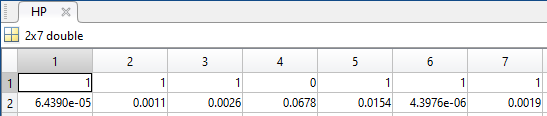
\includegraphics[width=0.68\textwidth]{HP}
	\caption{Rezultati Pirsonovog hi-kvadrat testa}
	\label{HP}
\end{figure}

Kao što se može videti sa \hyperref[HP]{gornje slike}, jedino je za četvrtu promenljivu, broj putnika, prihvaćena nulta hipoteza.

U nastavku je ispitivana efikasnost avio kompanije u popunjavanju dostupnih sedišta, pa je sedma promenljiva uzeta za zavisnu, a ostale promenljive za nezavisne.

\newpage

\thispagestyle{empty}

\section{Jednostruki linearni model}

\setcounter{footnote}{0}

Kao što je viđeno u prethodnom poglavlju (\hyperref[Rho]{Slika \ref*{Rho}}), sedma promenljiva ima najveći koeficijent korelacije sa petom promenljivom.\ Stoga, posmatra se jednostruki linearni model \[Y = \beta_0 + \beta_1 x_5 + \varepsilon ,\] gde je zavisna promenjiva $Y$ procenat zauzetih sedišta, nezavisna promenljiva $x_5$ broj putničkih kilometara u hiljadama, $\beta_0$ i $\beta_1$ parametri koje treba oceniti i $\varepsilon$ slučajna greška.

Ocene parametara $\beta_0$ i $\beta_1$ su dobijene metodom najmanjih kvadrata koji je izveden u \hyperref[OT]{Dodatku \ref*{OT}}.\ Takođe, za svaki tako dobijeni linearni model sa odsečkom (eng.\ \textit{intercept}) se u daljem tekstu pretpostavlja da je očekivana vrednost slučajne greške jednaka nuli.\ Jednačina linearne regresije jedno-strukog modela za procenat zauzetih sedišta preko broja putničkih kilometara u hiljadama je \[\hat{Y} = 41.93899569 + 0.00003381 x_5.\]

Dijagram rasipanja i regresiona prava su prikazani na \hyperref[jm]{Slici \ref*{jm}}.

\begin{figure}[h!]
	\centering
	\captionsetup{justification=centering}
	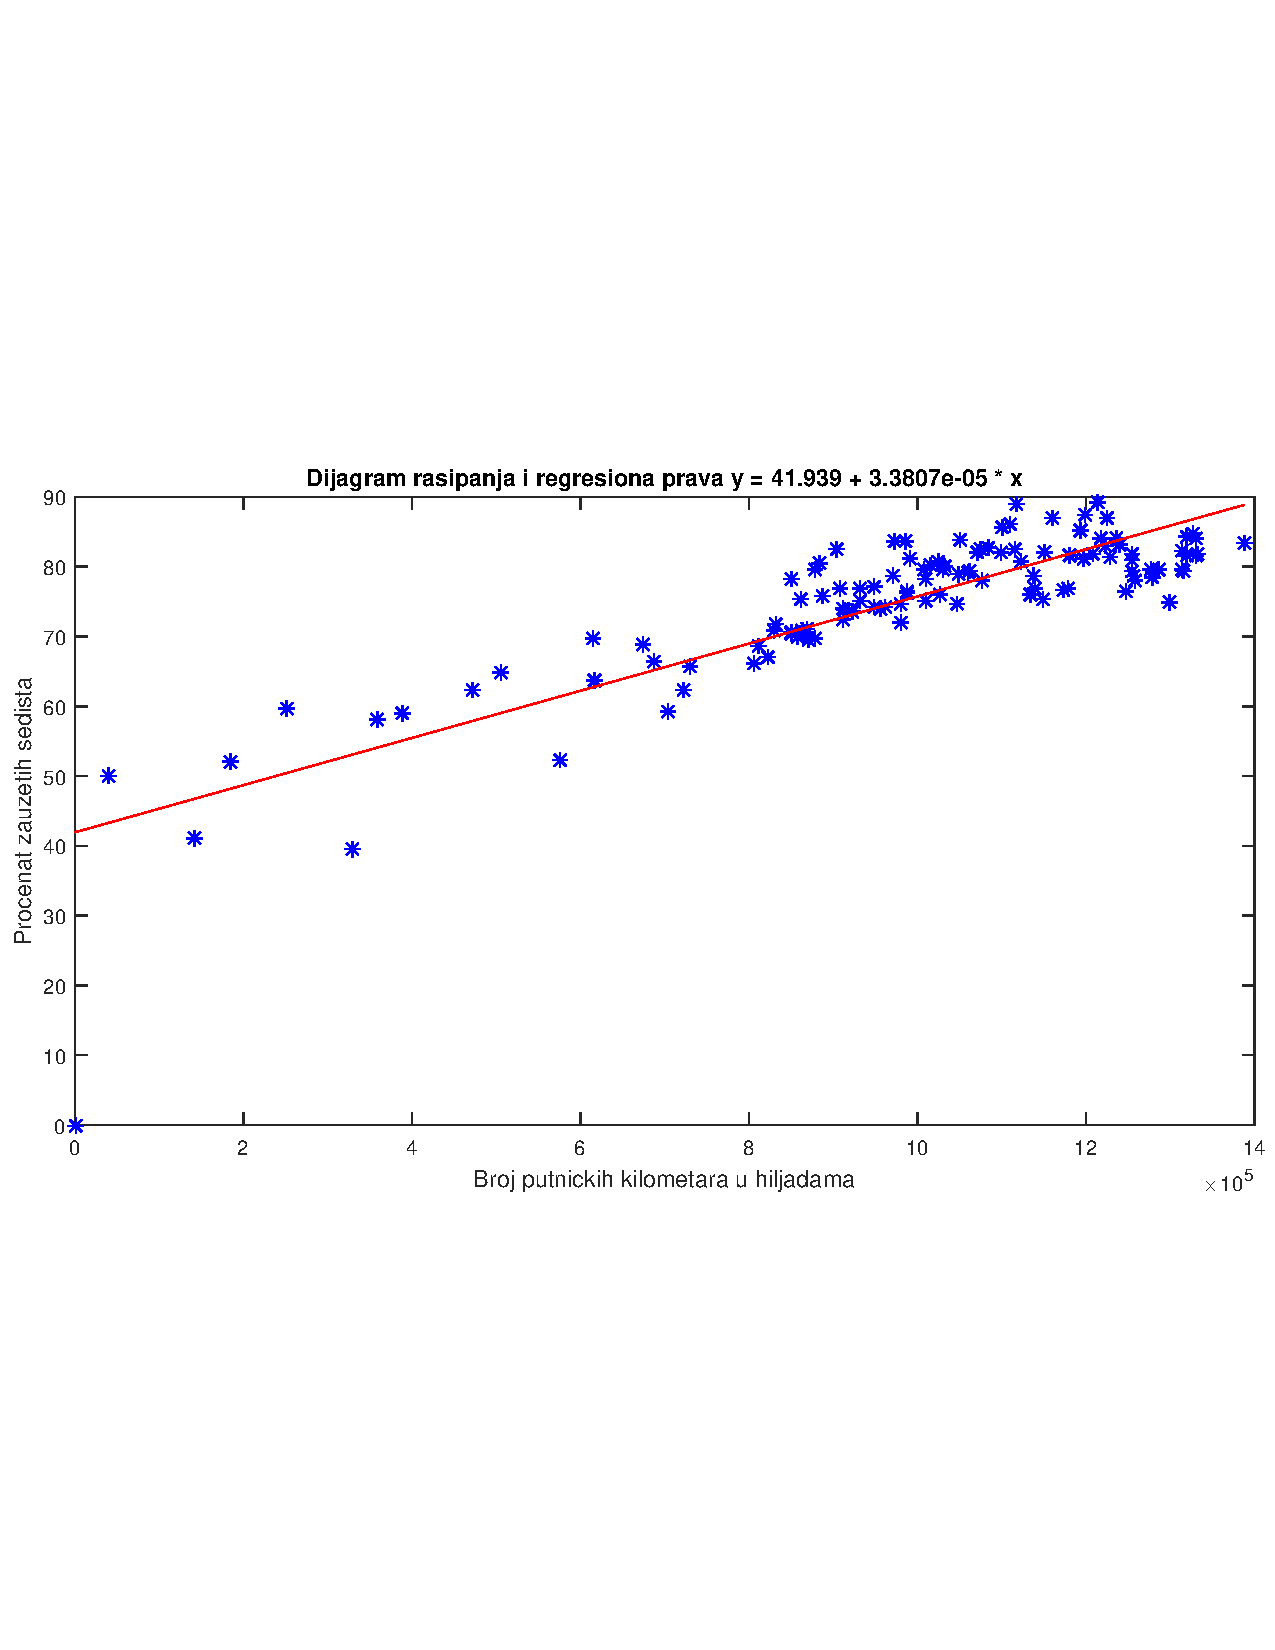
\includegraphics[width=0.98\textwidth]{jm}
	\caption{Dijagram rasipanja i regresiona prava jednostrukog linearnog modela}
	\label{jm}
\end{figure}

Bitna pretpostavka nekih statističkih testova i intervala poverenja je da reziduali imaju normalnu raspodelu.\ Odavde sledi da bi podaci nezavisne promenljive trebali da budu saglasni sa njom.\ Kao što je viđeno na kraju \hyperref[Uvod]{prethodnog poglavlja}, ova pretpostavka nije ispunjena na nivou značajnosti $0.05$.\ S obzirom na to, zaključke i rezultate kod kojih ova pretpostavka igra bitnu ulogu treba uzeti sa rezervom.

Ispunjenost pretpostavke o homoskedastičnosti reziduala je ispitana pomoću studentizovanog Bruš-Peiganovog testa (videti \cite{BrP, Ko}).\ Za njegovu implementaciju u Matlab-u videti \hyperref[bptest]{Algoritam \ref*{bptest}}.\ Pošto je izabrana studentizovana verzija, pretpostavlja se da su greške nezavisne i identično raspodeljene\footnote{u originalnoj verziji se pretpostavlja da je raspodela normalna}.\ Nulta hipoteza ovog testa je da su reziduali homoskedastični, a alternativna hipoteza je da su oni heteroskedastični (tj.\ nisu homoskedastični).\ Dobijena $p$-vrednost je $2.0505\cdot 10^{-4}$, što je (strogo) manje od $0.05$, pa se na nivou poverenja $0.95$ zaključuje da su reziduali heteroskedastični.

Dijagram rasipanja reziduala posmatranog modela u odnosu na ocenu zavisne promenljive je prikazan na \hyperref[res_vs_fitted_jm]{Slici \ref*{res_vs_fitted_jm}}.\ Sa nje se takođe može primetiti heteroskedastičnost reziduala.

\begin{figure}[h!]
	\centering
	\captionsetup{justification=centering}
	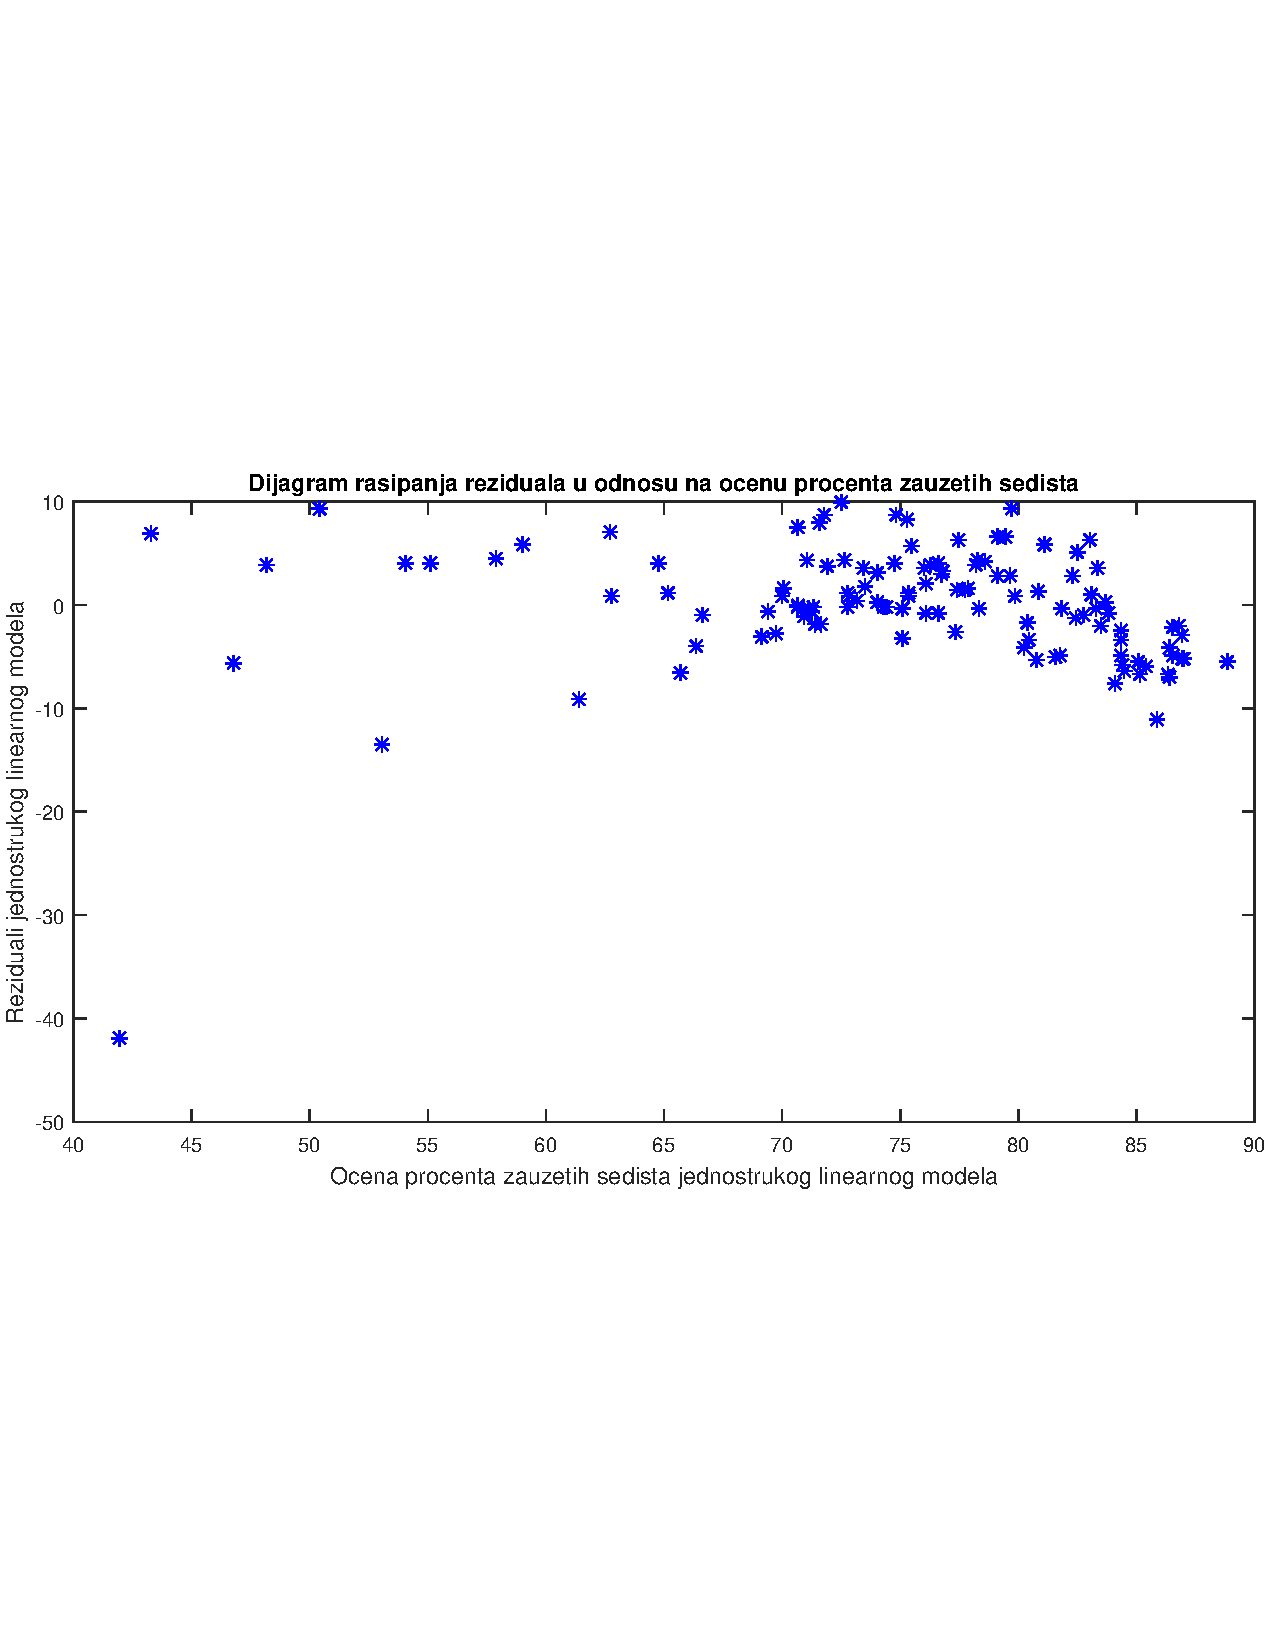
\includegraphics[width=0.98\textwidth]{res_vs_fitted_jm}
	\caption{Dijagram rasipanja reziduala jednostrukog linearnog modela}
	\label{res_vs_fitted_jm}
\end{figure}

Interval poverenja na nivou $0.95$ za parametar $\beta_0$ je \[\left[\hat{\beta}_0 - q\sqrt{\hat{D}(\hat{\beta}_0)},\,\hat{\beta}_0 + q\sqrt{\hat{D}(\hat{\beta}_0)}\right],\] gde je $\hat{\beta}_0$ ocena parametra $\beta_0$, $q$ kvantil reda $0.975$ Studentove raspodele sa $n - 2$ stepeni slobode i $\hat{D}(\hat{\beta}_0)$ ocena disperzije $\hat{\beta}_0$.\ Dobijeni interval poverenja na nivou $0.95$ za parametar $\beta_0$ je \[[38.00572262, 45.87226876].\] Analogno, interval poverenja na nivou $0.95$ za parametar $\beta_1$ je \[\left[\hat{\beta}_1 - q\sqrt{\hat{D}(\hat{\beta}_1)},\,\hat{\beta}_1 + q\sqrt{\hat{D}(\hat{\beta}_1)}\right],\] gde je $\hat{\beta}_1$ ocena parametra $\beta_1$, $q$ kvantil reda $0.975$ Studentove raspodele sa $n - 2$ stepeni slobode i $\hat{D}(\hat{\beta}_1)$ ocena disperzije $\hat{\beta}_1$.\ Dobijeni interval poverenja na nivou $0.95$ za parametar $\beta_1$ je \[[0.00002995, 0.00003767].\] Da bi se odredili intervali poverenja za parametre $\beta_0$ i $\beta_1$, potrebno je da važi pretpostavka o homoskedastičnosti reziduala i da oni imaju normalnu raspodelu.\ Kako to nije ispunjeno, ne može se tvrditi da su dobijeni intervali poverenja odgovarajući.

Srednja kvadratna greška (eng.\ \textit{mean squared error}) je definisana sa $MSE = RSS/n$, gde je $RSS$ suma kvadrata reziduala.\ Kako je minimizacija srednje kvadratne greške ekvivalentna minimizaciji sume kvadrata reziduala, ona je u daljem tekstu korišćena za evaluaciju modela.\ U ovom slučaju ona iznosi $35.9167$.

Koeficijent determinacije je $0.7201$.\ Pošto je on blizu $1$, može se reći da je
veći deo varijabilnosti zavisne promenljive objašnjen modelom.

Pored ovog, nađeni su i ostali jednostruki linearni modeli sa odsečkom.\ Za sve njih je utvrđeno da postoji linearna veza između odgovarajuće nezavisne promenljive i procenta zauzetih sedišta, na nivou poverenja $0.95$.\ Naravno, ove rezultate treba uzeti sa rezervom, jer samo broj putnika ima normalnu raspodelu i reziduali su u svim slučajevima heteroskedastični prema studentizovanom Bruš-Peiganovom testu, oba na nivou poverenja $0.95$.\ Dodatno, izračunate su srednje kvadratne greške i koeficijenti determinacije svih modela, gde se kao najbolji pokazao model predstavljen u ovom poglavlju.\ S obzirom na to da je koeficijent determinacije jednak kvadratu uzoračkog koeficijenta korelacije, ovaj rezultat je bio očekivan (videti i \hyperref[posledica]{Posledicu \ref*{posledica}}\,(i)).

\newpage

\thispagestyle{empty}

\section{Pun linearni model}

\setcounter{footnote}{0}

Kako postoji linearna veza između datih promenljivih, posmatra se višestruki linearni model \[Y = \beta_0 + \beta_1 x_1 + \beta_2 x_2 + \beta_3 x_3 + \beta_4 x_4 + \beta_5 x_5 + \beta_6 x_6 + \varepsilon ,\] gde su sa $x_1$ do $x_6$ označene nezavisne promenljive tim redom kojim se javljaju na listi sa početka \hyperref[Uvod]{Poglavlja \ref*{Uvod}}, zavisna promenjiva $Y$ je procenat zauzetih sedišta, $\beta_0$ do $\beta_6$ su parametri koje treba oceniti i $\varepsilon$ slučajna greška.

Neka su sa $X_1$ do $X_6$ označeni odgovarajući uzorci nezavisnih promenljivih $x_1$ do $x_6$, respektivno.\ Tada je rang matrice $X = [1_{n\times 1}~X_1~\dots~X_6]$ jednak $7$.\ Odavde sledi da se parametri linearne regresije koja modeluje procenat zauzetih sedišta preko ostalih šest promenljivih i odsečka, ili bilo kog njihovog podskupa, mogu oceniti na jedinstven način metodom najmanjih kvadrata.

Tako je dobijena jednačina linearne regresije punog modela za procenat zauzetih sedišta preko ostalih promenljivih
\begin{gather*}
\hat{Y} = 43.79588813 + 0.00552488 x_1 - 0.00141099 x_2 + 0.00149182 x_3\\
-\phantom{.}0.00009411 x_4 + 0.00016416 x_5 - 0.00005799 x_6.
\end{gather*}

Studentizovani Bruš-Peiganov test daje $p$-vrednost $2.8601\cdot 10^{-5}$, što je (strogo) manje od $0.05$, pa se na nivou poverenja $0.95$ zaključuje da su reziduali heteroskedastični.

\begin{figure}[h!]
	\centering
	\captionsetup{justification=centering}
	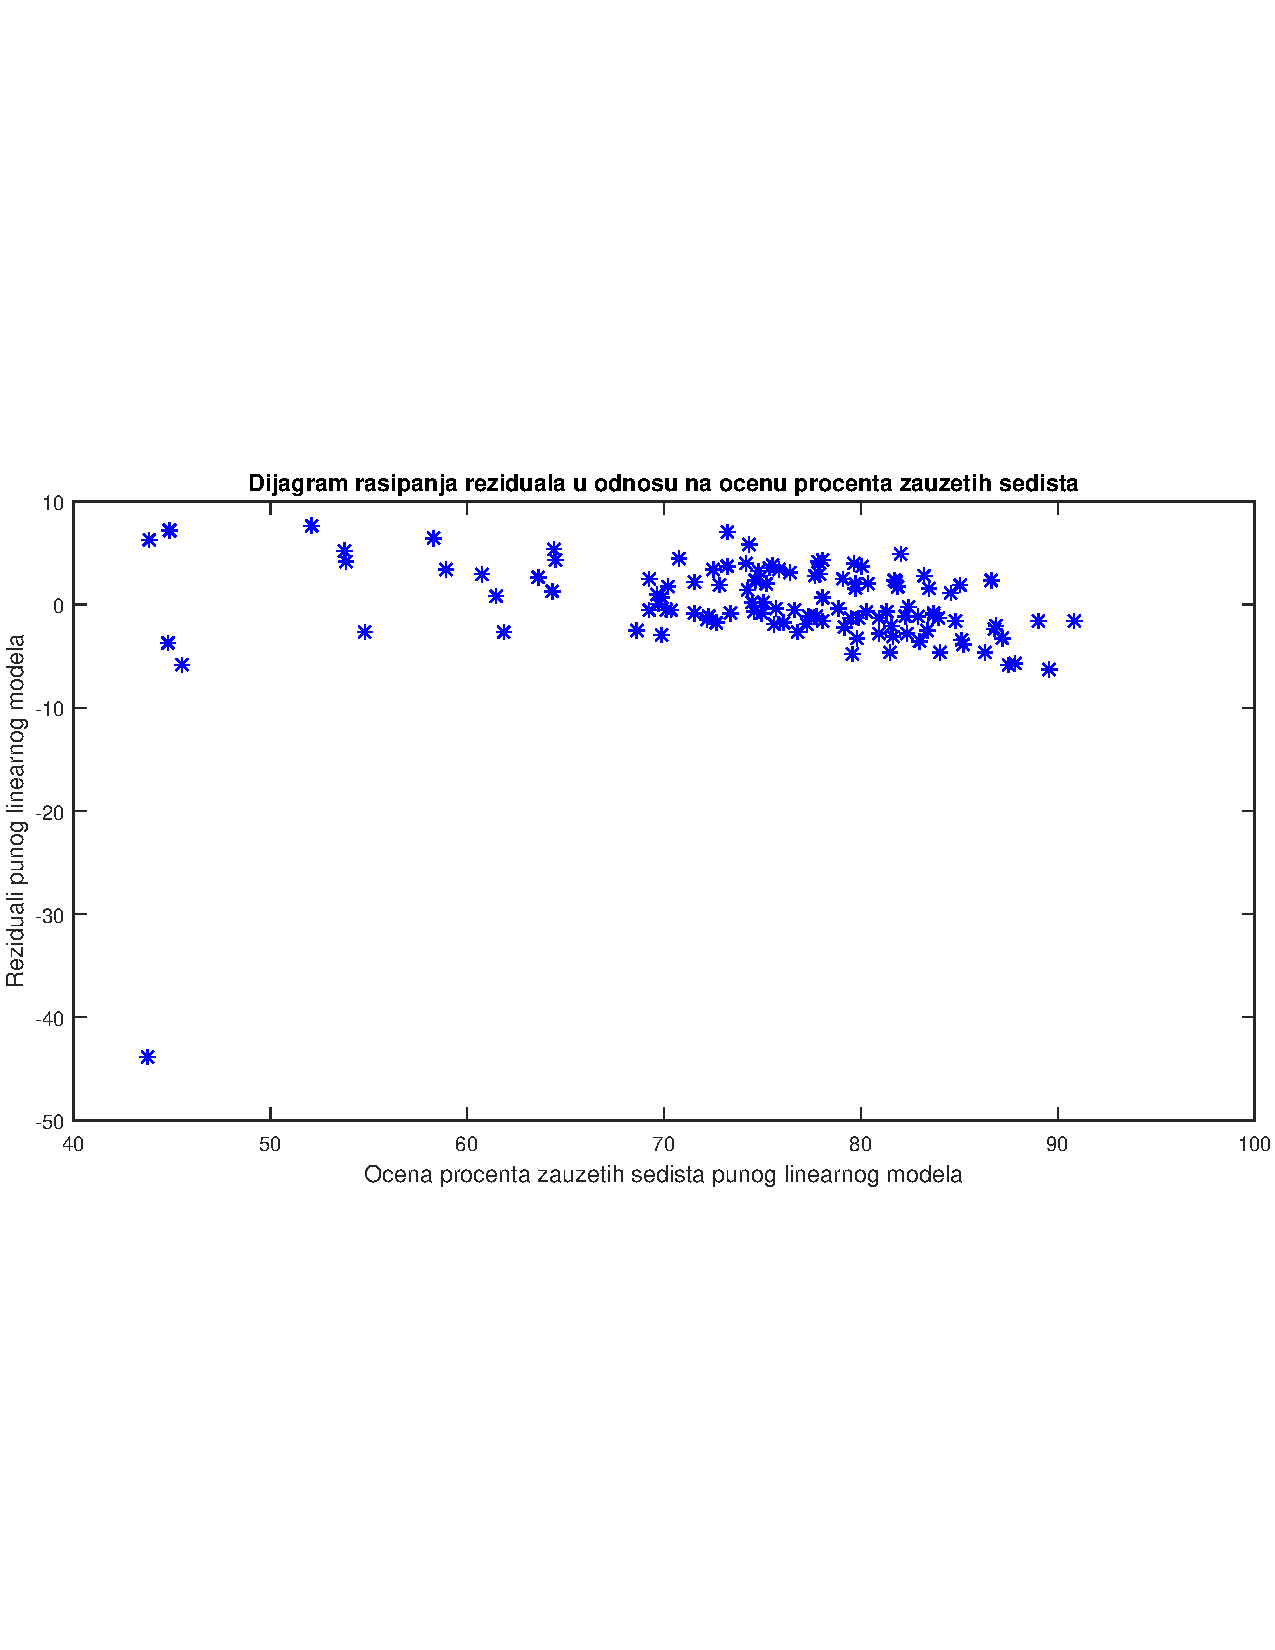
\includegraphics[width=0.9784\textwidth]{res_vs_fitted}
	\caption{Dijagram rasipanja reziduala punog linearnog modela}
	\label{res_vs_fitted}
\end{figure}

Na \hyperref[res_vs_fitted]{Slici \ref*{res_vs_fitted}} je prikazan dijagram rasipanja reziduala posmatranog modela u odnosu na ocenu zavisne promenljive.

Srednja kvadratna greška ovog modela je $25.8121$, a koeficijent determinacije je $0.7989$, što je dosta bolje od jednostrukog modela.\ Očekivano, koeficijent determinacije raste sa porastom broja promenljivih (\hyperref[R2]{Posledica \ref*{R2}}).

\newpage

\thispagestyle{empty}

\section{Redukovani linearni model}\label{Redukovani linearni model}

\setcounter{footnote}{0}

Čest problem punog modela je taj što on može da sadrži nezavisne pro-menljive koje nisu relevantne ili su redundantne.\ U tom slučaju je potrebno uzeti podskup datih promenljivih takav da model dobijen preko njih ima slične performanse.\ Na ovaj način se uspešnim odabirom promenljivih mogu izbeći problemi koji se javljaju u višedimenzionalnim prostorima, ubrzati izračunavanja i poboljšati predviđanja \cite{urlcv}.

Postoje razni algoritmi za odabir promenljivih.\ Jedan od njih je „odabir odlika ka napred” (eng.\ \textit{forward feature selection}), koji je ovde primenjen za linearni model i ocenu performansi preko sume kvadrata reziduala.\ Ovaj algoritam polazi od modela koji sadrži samo odsečak.\ Nakon toga se traži promenljiva takva da njenim dodavanjem novodobijeni model ima najmanju sumu kvadrata reziduala.\ Da bi model dobijen na takav način bio izabran, neophodno je da njegova suma kvadrata reziduala bude značajno manja od sume kvadrata reziduala prethodno izabranog modela.\ U tu svrhu se radi F-test.\ Ako je razlika suma kvadrata reziduala statistički značajna, onda posmatranu promenljivu dodajemo u skup izabranih.\ Ovaj postupak se ponavlja do prve razlike koja nije statistički značajna, ili dok se ne iskoriste sve promenljive.

Preciznije, ako je $RSS$ suma kvadrata reziduala izabranog modela, a $RSS_c$ suma kvadrata reziduala novog modela dobijenog dodavanjem jedne, do sada nekorišćene, promenljive, onda važi \[\dfrac{RSS - RSS_c}{\dfrac{RSS_c}{n - k}}: F_{1, n - k},\] ako reziduali imaju normalnu raspodelu, gde je $k$ broj ocenjenih parametara novog modela.\ Za implementaciju u Matlab-u videti \hyperref[ffsb]{Algoritam \ref*{ffsb}}.

Kao što je već rečeno, pošto nije ispunjena pretpostavka o normalnoj raspodeli reziduala, rezultate gornjeg statističkog testa treba uzeti sa rezervom.

Neka je procenat zauzetih sedišta zavisna promenljiva, ostale promenljive nezavisne i nivo značajnosti $0.05$.\ Promenljive izabrane primenom ovog algoritma su broj putničkih kilometara u hiljadama, broj sati letenja i broj putnika, tim redom.

Prema tome, posmatra se višestruki linearni model \[Y = \beta_0 + \beta_1 x_5 + \beta_2 x_2 + \beta_3 x_4 + \varepsilon ,\] gde su $x_5$, $x_2$ i $x_4$ nezavisne promenljive u gore navedenom redosledu, zavis-na promenljiva $Y$ procenat zauzetih sedišta, $\beta_0$ do $\beta_3$ parametri koje treba oceniti i $\varepsilon$ slučajna grešaka.\ Metodom najmanjih kvadrata su dobijene ocene parametara $\beta_0$ do $\beta_3$.\ Jednačina linearne regresije redukovanog modela za procenat zauzetih sedišta preko izabranih promenljivih je \[\hat{Y} = 44.07230816 + 0.00011081 x_5 - 0.00177392 x_2 - 0.00005108 x_4.\]

Primenom studentizovanog Bruš-Peiganovog testa se dobija $p$-vrednost $1.2182\cdot 10^{-5}$, što je (strogo) manje od $0.05$, pa se na nivou poverenja $0.95$ zaključuje da su reziduali heteroskedastični.

Dijagram rasipanja reziduala redukovanog linearnog modela u odnosu na ocenu zavisne promenljive je prikazan na \hyperref[res_vs_fitted_red]{Slici \ref*{res_vs_fitted_red}}.

\begin{figure}[h!]
	\centering
	\captionsetup{justification=centering}
	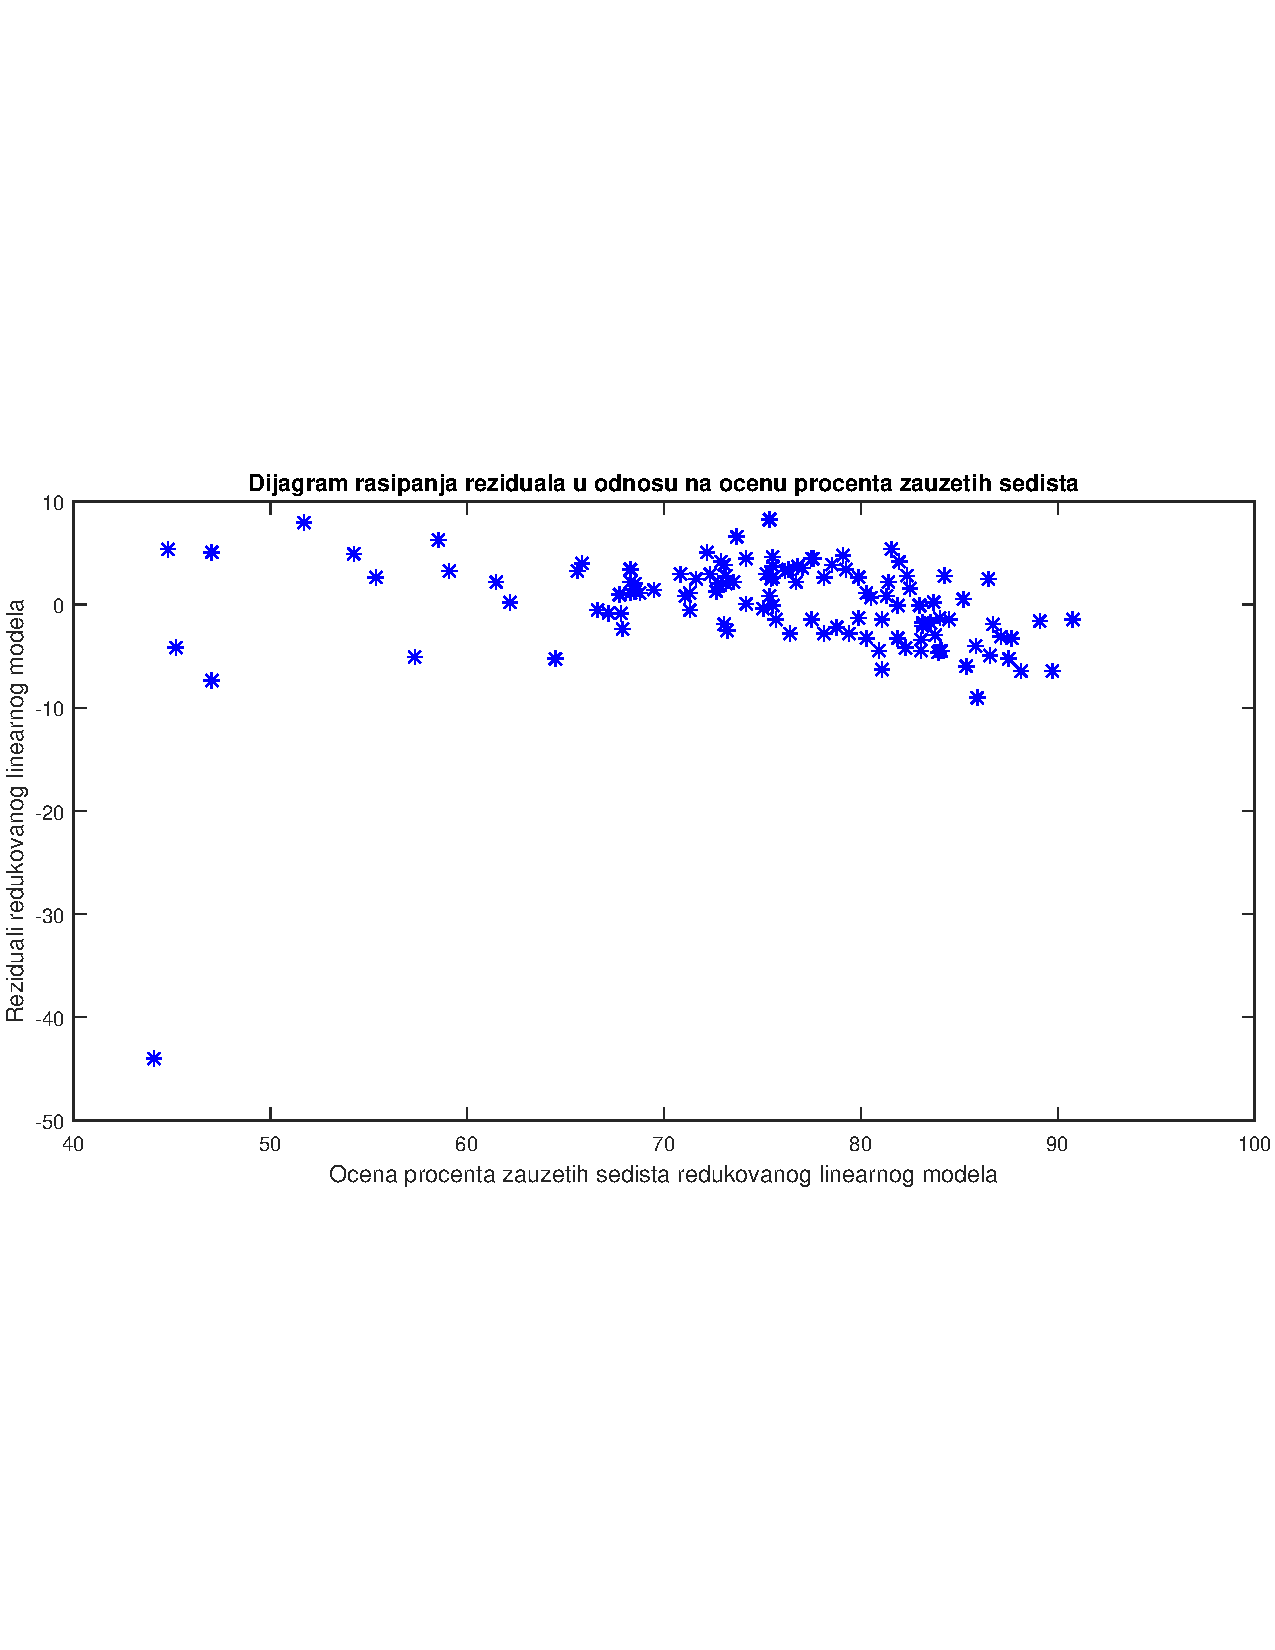
\includegraphics[width=0.98\textwidth]{res_vs_fitted_red}
	\caption{Dijagram rasipanja reziduala redukovanog linearnog modela}
	\label{res_vs_fitted_red}
\end{figure}

Srednja kvadratna greška ovog modela je $28.7738$, a koeficijent determinacije je $0.7758$, što je malo lošije od punog modela.

Prirodno se postavlja pitanje da li pun model daje značajno bolje ocene zavisne promenljive od redukovanog modela.\ Da bi se to ispitalo, testira se nulta hipoteza $H_0 (\beta^{izb} = 0_{h\times 1})$, gde je $\beta^{izb}$ vektor parametara koji su izbačeni iz punog modela i $h$ njihov broj, protiv alternativne $H_1 (\beta^{izb} \neq 0_{h\times 1})$, koristeći test statistiku \[\dfrac{\dfrac{RSS^{red} - RSS}{h}}{\dfrac{RSS}{n - k}} = F_{reg},\] gde je $RSS^{red}$ suma kvadrata reziduala redukovanog, a $RSS$ punog modela i $k$ broj ocenjenih parametara punog modela.\ Nulta hipoteza $H_0 (\beta^{izb} = 0_{h\times 1})$ se odbacuje ako je $F_{reg} > q$, gde je $q$ kvantil reda $0.95$ Fišerove raspodele sa $h$ i $n - k$ stepeni slobode.\ U ovom slučaju je $h = 3$, $n - k = 112$ i $F_{reg} = 4.2837 > 2.6856 = q$.\ To znači da se nulta hipoteza $H_0 (\beta^{izb} = 0_{h\times 1})$ odbacuje na nivou poverenja $0.95$, odnosno pun model pruža značajno bolje prilagođavanje podacima od redukovanog modela.

\newpage

\thispagestyle{empty}

\section{Nelinearni modeli}\label{Nelinearni modeli}

\setcounter{footnote}{0}

Pošto procenat zauzetih sedišta može da uzima vrednosti samo između $0$ i $100$, a linearna funkcija nije ograničena, linearni modeli daju vrednosti van tog intervala, što nema realnog smisla (videti \cite{Ri} za poznati primer sa sličnim problemom).\ Ovo motiviše pravljenje regresionog modela pomoću nelinearne funkcije.\ Poželjno je da ona uzima vrednosti samo od $0$ do $100$ i da joj domen nije ograničen odozgo (jer ostale nezavisne promenljive nisu ograničene odozgo).\ Ne postoji egzaktna procedura za odabir funkcije, pa intuicija za njen izbor dolazi i sa dijagrama rasipanja (videti \hyperref[jm]{Sliku \ref*{jm}}).

Jedna funkcija koja odgovara gornjem opisu je \[L(x) = \dfrac{100}{1 + e^{-x}},\] čija je skica grafika data na \hyperref[nlin]{Slici \ref*{nlin}}, gde je $y = L(x)$.

\begin{figure}[h!]
	\centering
	\captionsetup{justification=centering}
	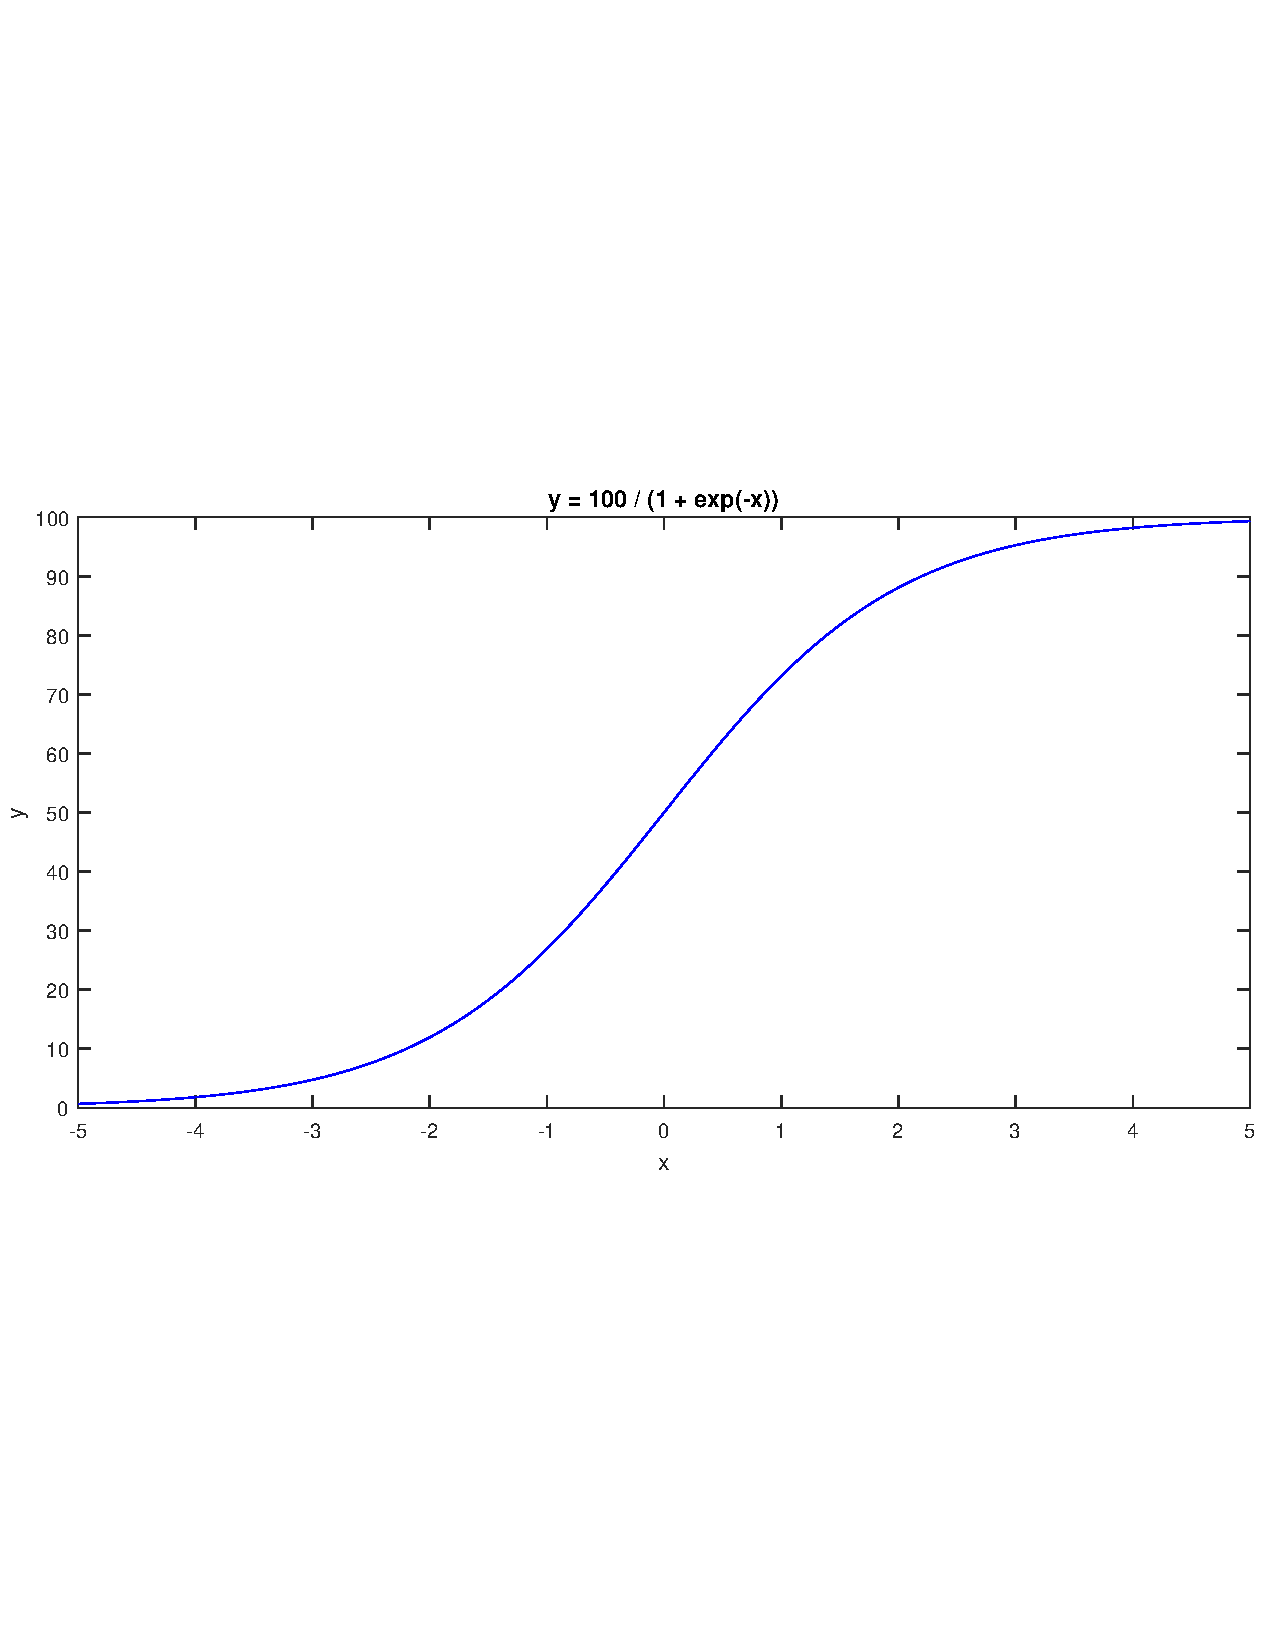
\includegraphics[width=0.98\textwidth]{nlin}
	\caption{Skica grafika $y = \dfrac{100}{1 + e^{-x}}$}
	\label{nlin}
\end{figure}

Kako je domen funkcije $L$ ceo skup realnih brojeva, njen argument može biti bilo koji realan broj, pa se može uzeti linearna kombinacija nezavisnih promenljivih i konstante.\ Konkretno, za jednostruki nelinearni model ta linearna kombinacija je $\beta_0 + \beta_1 x_5$, gde je $x_5$ broj putničkih kilometara u hiljadama, a $\beta_0$ i $\beta_1$ su parametri koje treba oceniti.\ Stoga, posmatra se jednostruki nelinearni model \[Y = L(\beta_0 + \beta_1 x_5) + \varepsilon = \dfrac{100}{1 + e^{-(\beta_0 + \beta_1 x_5)}} + \varepsilon ,\] gde je zavisna promenjiva $Y$ procenat zauzetih sedišta i $\varepsilon$ slučajna greška.

Ocene parametara $\beta_0$ i $\beta_1$ su dobijene metodom najmanjih kvadrata koristeći Gaus-Njutnov postupak (za više detalja videti \cite{urlFl}).\ Prilikom njegove primene, parcijalni izvodi u Jakobijanu su aproksimirani pomoću numeričkog postupka koji se naziva diferenciranje kompleksnim korakom (eng.\ \textit{Complex Step Differentiation}).\ Naime, ako su $r_i$, $i\in\lbrace 1, 2, \dots , n\rbrace$, holomorfne funkcije\footnote{tj.\ funkcije koje su kompleksno diferencijabilne u svakoj tački posmatranog otvorenog skupa} koje uzimaju realne vrednosti za $\bm{x}\in\mathbb{R}^k$, $\bm{r} = [r_1~r_2~\dots ~r_n]^T$ i $J_{\bm{r}}(\bm{x})$ Jakobijan od $\bm{r}$ u tački $\bm{x}$, onda važi
\[
J_{\bm{r}}(\bm{x})
\approx \frac{1}{h}\mathop{\mathfrak{Im}}
\begin{bmatrix}
	r_1(\bm{x} + ih\bm{e_1}) & r_1(\bm{x} + ih\bm{e_2}) & \dots  & r_1(\bm{x} + ih\bm{e_k}) \\
	r_2(\bm{x} + ih\bm{e_1}) & r_2(\bm{x} + ih\bm{e_2}) & \dots  & r_2(\bm{x} + ih\bm{e_k}) \\
	\vdots & \vdots &  & \vdots \\
	r_n(\bm{x} + ih\bm{e_1}) & r_n(\bm{x} + ih\bm{e_2}) & \dots  & r_n(\bm{x} + ih\bm{e_k})
\end{bmatrix}
,
\]
gde je $h$ korak, $\bm{e_j}$ $j$-ta kolona jedinične matrice $\bm{E_{k\times k}}$, $j\in\lbrace 1, 2, \dots , k\rbrace$, i $\mathop{\mathfrak{Im}}$ imaginarni deo kompleksnog broja.\ Dokaz prethodnog se može naći, na primer, u \cite{LaC}.\ Za implementaciju Gaus-Njutnovog postupka (gde je korišćena navedena aproksimacija parcijalnih izvoda) u Matlab-u videti \hyperref[gn]{Algoritam \ref*{gn}}.

Jasno je da se gore navedeno može primeniti na posmatrani model da bi se dobile ocene parametara $\beta_0$ i $\beta_1$.\ Neka je $\beta = [\beta_0 ~\beta_1]^T$.\ Uzimajući~za početak Gaus-Njutnovog postupka $\hat{\beta}_{(0)} = 0_{2\times 1}$, korak aproksimacije parci-jalnih izvoda $h = 10^{-11}$, maksimalan broj iteracija $100$ i uslov zaustavlja-nja $\norm{\hat{\beta}_{(s)} - \hat{\beta}_{(s + 1)}}_2 < 10^{-11}$, gde je sa $(s)$ u indeksu označen $s$-ti korak, $s\in\lbrace 0, 1, \dots , 99\rbrace$, dobija se
\[
\hat{\beta} =
\begin{bmatrix}
	-0.52146894\\
	\mathbin{\phantom{+}}0.00000172
\end{bmatrix}
.
\]
Dakle, jednačina nelinearne regresije jednostrukog modela za procenat zauzetih sedišta preko broja putničkih kilometara u hiljadama je \[\hat{Y} = \dfrac{100}{1 + e^{0.52146894 - 0.00000172 x_5}}.\]

Dijagram rasipanja i regresiona kriva su prikazani na \hyperref[jm_nlin]{Slici \ref*{jm_nlin}}.

\begin{figure}[h!]
	\centering
	\captionsetup{justification=centering}
	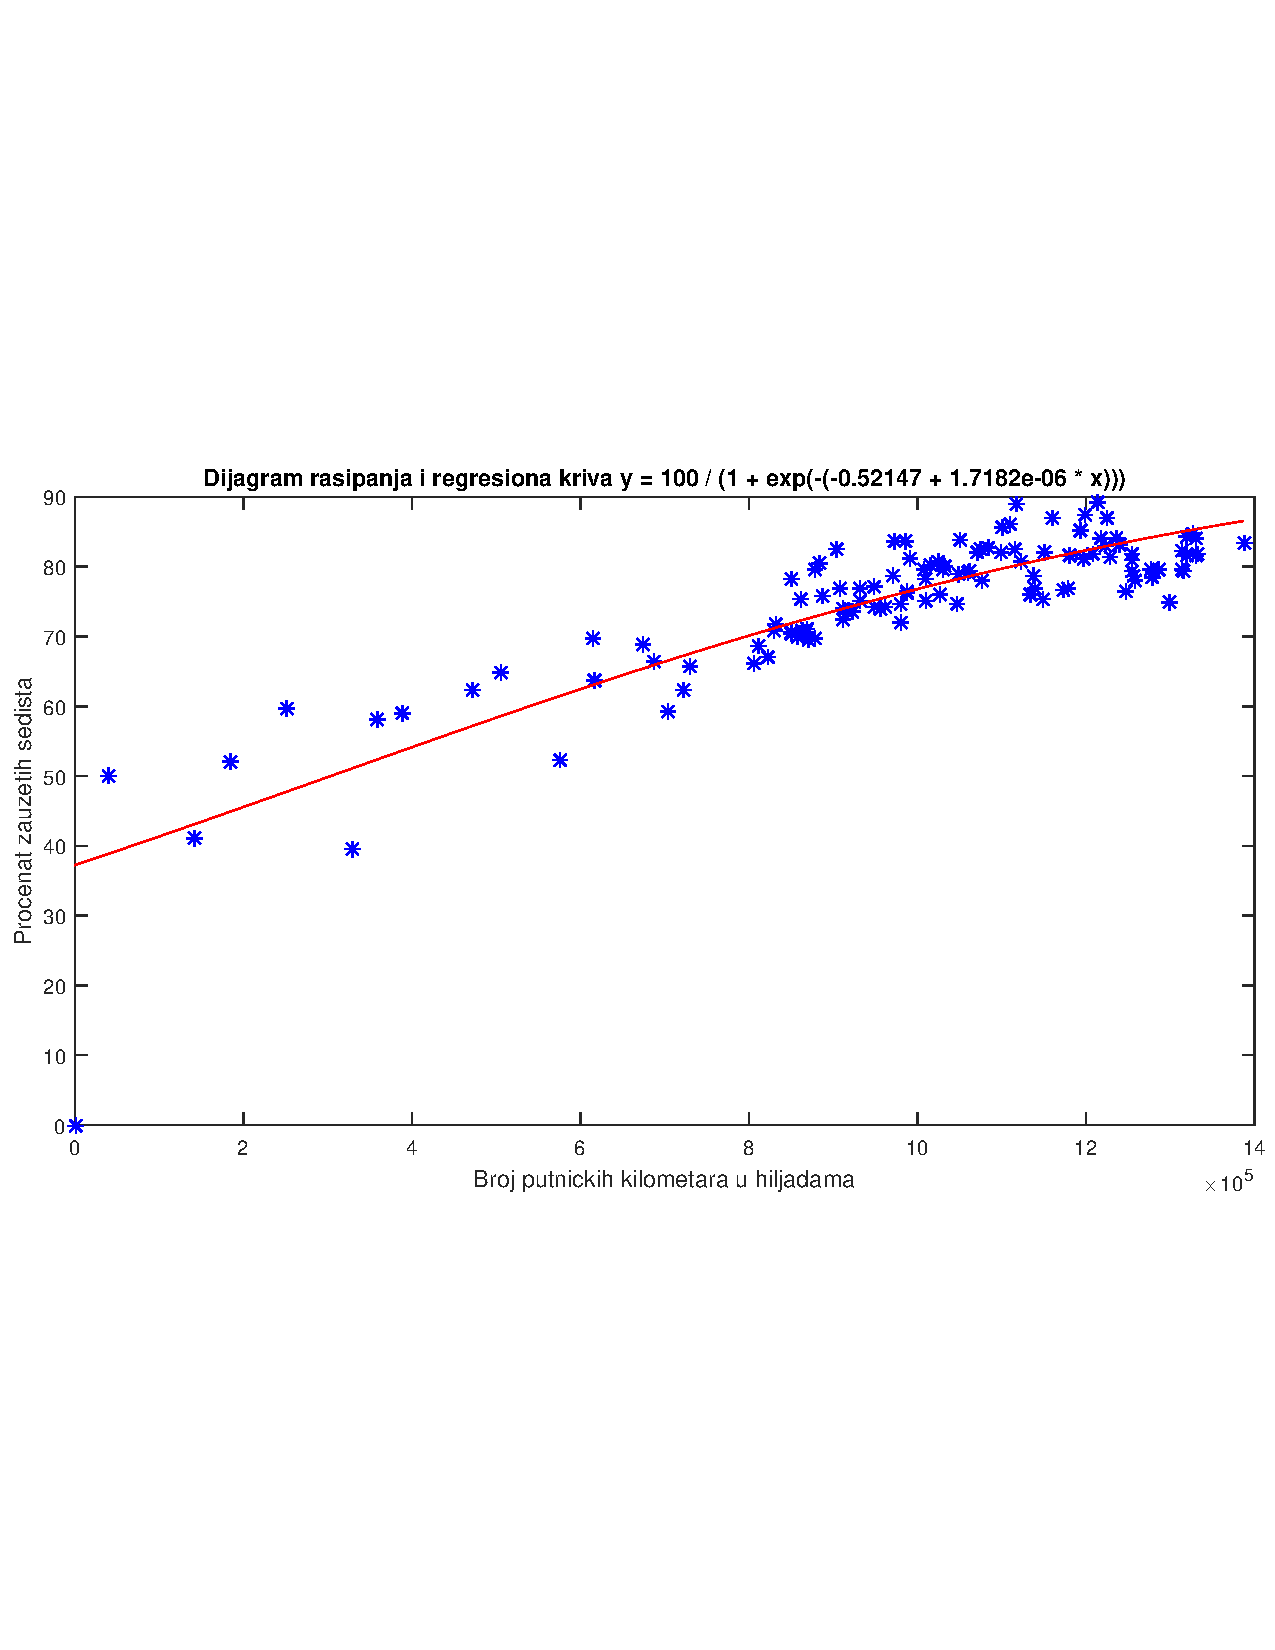
\includegraphics[width=0.98\textwidth]{jm_nlin}
	\caption{Dijagram rasipanja i regresiona kriva jednostrukog nelinearnog modela}
	\label{jm_nlin}
\end{figure}

Srednja kvadratna greška jednostrukog nelinearnog modela je $30.7402$, što je bolje od odgovarajućeg linearnog modela.

Analogno, posmatraju se pun i redukovani višestruki nelinearni modeli
\begin{gather*}
	Y = \dfrac{100}{1 + e^{-(\beta_0 + \beta_1 x_1 + \beta_2 x_2 + \beta_3 x_3 + \beta_4 x_4 + \beta_5 x_5 + \beta_6 x_6)}} + \varepsilon ,\\
	Y = \dfrac{100}{1 + e^{-(\beta_0 + \beta_1 x_5 + \beta_2 x_2 + \beta_3 x_4)}} + \varepsilon ,
\end{gather*}
respektivno, gde su sa $x_1$ do $x_6$ označene nezavisne promenljive tim redom kojim se javljaju na listi sa početka \hyperref[Uvod]{Poglavlja \ref*{Uvod}}, zavisna promenjiva $Y$ je procenat zauzetih sedišta, u prvom slučaju $\beta_0$ do $\beta_6$, a u drugom $\beta_0$ do $\beta_3$, su parametri koje treba oceniti i $\varepsilon$ slučajna greška, u oba slučaja.\ Bitno je napomenuti da redukovani nelinearni model koristi nezavisne promenljive izabrane u \hyperref[Redukovani linearni model]{prethodnom poglavlju} za redukovani linearni model.\ Dakle, nije vršena redukcija koja odgovara nelinearnom modelu.

Ocene parametara oba modela su dobijene metodom najmanjih kvadrata koristeći Gaus-Njutnov postupak na isti način kao kod ocene parametara jed-nostrukog nelinearnog modela.\ Jednačina nelinearne regresije punog modela za procenat zauzetih sedišta preko ostalih promenljivih je
\begin{gather*}
\hat{Y} = 100 / (1 + \exp(0.35680833 - 0.00019237 x_1 + 0.00006123 x_2\\
-\phantom{.}0.00009314 x_3 + 0.00000424 x_4 - 0.00000782 x_5 + 0.00000269 x_6)).
\end{gather*}
Jednačina nelinearne regresije redukovanog modela za procenat zauzetih sedišta preko promenljivih izabranih u \hyperref[Redukovani linearni model]{prethodnom poglavlju} je \[\hat{Y} = \dfrac{100}{1 + e^{0.35221238 - 0.00000559 x_5 + 0.00010635 x_2 + 0.00000236 x_4}}.\]

Srednja kvadratna greška punog nelinearnog modela je $22.5393$, a redukovanog je $24.1371$, što je u oba slučaja bolje od odgovarajućih linearnih modela.

Pošto nije vršena redukcija nezavisnih promenljivih koja odgovara neline-arnom modelu, može se desiti da je slobodan član u eksponentu suvišan za unapred dat podskup nezavisnih promenljivih.\ To će biti ispitano samo u slučaju nezavisnih promenljivih izabranih za redukovani linearni model, a rezultat ove odluke će biti evaluiran u \hyperref[Trening i testiranje]{sledećem poglavlju}.\ Prema tome, posmatra se redukovani višestruki nelinearni model bez slobodnog člana \[Y = \dfrac{100}{1 + e^{-(\beta_1 x_5 + \beta_2 x_2 + \beta_3 x_4)}} + \varepsilon ,\] gde su oznake iste kao malopre.

Ocene parametara su dobijene metodom najmanjih kvadrata koristeći Gaus-Njutnov postupak na isti način kao u prethodna tri slučaja.\ Jednačina nelinearne regresije redukovanog modela bez slobodnog člana za procenat zauzetih sedišta preko broja putničkih kilometara u hiljadama, broja sati letenja i broja putnika, tokom meseca, je \[\hat{Y} = \dfrac{100}{1 + e^{-0.00000514 x_5 + 0.00015471 x_2 + 0.00000152 x_4}}.\]

Srednja kvadratna greška redukovanog nelinearnog modela bez slobodnog člana je $26.8485$.

\newpage

\thispagestyle{empty}

\section{Trening i testiranje}\label{Trening i testiranje}

\setcounter{footnote}{0}

Podela podataka na trening i testiranje se koristi da bi se ocenile performanse predviđanja modela.\ Takođe, na ovaj način mogu da se uporede performanse predviđanja više modela.

Skup svih dostupnih podataka se, na slučajan način, deli na dva dela.\ Prvi deo, koji se uglavnom uzima da bude oko $70\%$ podataka, služi za pravljenje modela, što se naziva trening ili obuka modela, a odgovarajući skup podataka se naziva trening skup ili skup za obuku.\ Drugi deo, koji čine preostali podaci, se ne koristi za obuku modela, umesto toga, na njemu se ocenjuju performanse modela dobijenog na trening skupu.\ Ovaj drugi deo podataka se naziva skup za testiranje.

Modeli se ovako koriste u praksi.\ Naime, oni se treniraju na skupu svi dostupnih podataka, a zatim se pomoću njih prave predviđanja za željene slučajeve koji ne moraju da se nalaze u tom skupu podataka.

Gore navedeni slučajan izbor podataka za trening skup se radi kako bi se osigurala njegova reprezentativnost datog skupa podataka, koji bi zauzvrat trebao da bude reprezentativan uzorak zapažanja iz domena posmatranog problema.\ Prilikom upoređivanja modela, neophodno je da se oni treniraju i testiraju na istim podskupovima datog skupa podataka.

Naravno, podela podataka na trening i testiranje ima smisla samo kada je dati skup podataka dovoljno velik \cite{urlBr}.

Pored uslova da je moguće da se napravi model na trening skupu i on evaluira na test skupu, ova procedura ne zahteva nikakve dodatne pretpostavke.\ Takođe, poželjno je da se ona ponovi više puta kako bi ocene performansi predviđanja bile što preciznije.

Konkretno, veličina datog skupa podataka je $n = 119$, pa se uzimanjem, na slučajan način, približno $70\%$ podataka za trening skup dobija da je on veličine $n_{trening} = 83$, pa je veličina test skupa $n_{test} = 36$.\ Trening i testiranje, na istim podacima, je urađeno za svih sedam modela iz prethodnih poglavlja.\ Procedura je ponovljena $1000$ puta, a performanse predviđanja su ocenjene aritmetičkom sredinom srednjih kvadratnih grešaka na test skupovima.\ Dobijeni rezultati su prikazani na \hyperref[mean_MSE_test]{Slici \ref*{mean_MSE_test}} za svih sedam modela u redosledu njihovog pojavljivanja.

\begin{figure}[h!]
	\centering
	\captionsetup{justification=centering}
	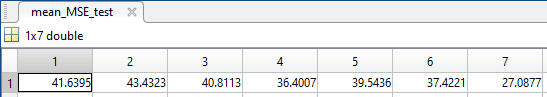
\includegraphics[width=0.68\textwidth]{mean_MSE_test}
	\caption{Aritmetička sredina srednjih kvadratnih grešaka na test skupovima}
	\label{mean_MSE_test}
\end{figure}

Kao što se može videti sa \hyperref[mean_MSE_test]{nje}, redukovani nelinearni model bez slobodnog člana ima najbolje performanse predviđanja, a za njim slede jednostruki nelinearni model, redukovani nelinearni model (sa slobodnim članom), pun nelinearni model, redukovani linearni model, jednostruki linearni model i pun linearni model, tim redom.\ Pored toga, svaki nelinearni model ocenjen je kao bolji od bilo kog linearnog.

Dakle, u praksi se za predviđanja koriste modeli dobijeni u prethodnim poglavljima na skupu svih dostupnih podataka, dok su njihove ocene performansi predviđanja date na \hyperref[mean_MSE_test]{Slici \ref*{mean_MSE_test}}.

Bitno je napomenuti da procenat podataka za trening skup, slučajnost pri njihovom izboru i broj iteracija utiču na krajnji rezultat ove procedure.

\newpage

\thispagestyle{empty}

\section{Zaključak}

\setcounter{footnote}{0}

Kako bi se predvidela efikasnost avio kompanije u popunjavanju dostupnih sedišta, posmatrana su sedam modela.\ Za sve njih su, između ostalog, nađene srednje kvadratne greške.\ Pored toga, kako bi se procenila njihova tačnost predviđanja, urađen je trening i testiranje gde je za ocenu performansi uzeta aritmetička sredina hiljadu srednjih kvadratnih grešaka.\ Prema tome, ima smisla uporediti ove rezultate.\ Oni su dati, na dve decimale, u \hyperref[tabela]{tabeli ispod} za svih sedam modela u redosledu njihovog pojavljivanja.\
\begin{table}[h!]
\begin{center}
\begin{tabular}{c c c c c c c c}
\Xhline{3\arrayrulewidth}
MSE & 35.92 & 25.81 & 28.77 & 30.74 & 22.54 & 24.14 & 26.85 \\
a.s.\ test MSE & 41.64 & 43.43 & 40.81 & 36.40 & 39.54 & 37.42 & 27.09 \\
\Xhline{3\arrayrulewidth}
\end{tabular}
\caption{Srednje kvadratne greške i njihove aritmetičke sredine na test skupovima za posmatrane modele}
\label{tabela}
\end{center}
\end{table}
Kao što se vidi sa \hyperref[tabela]{nje}, ocene performansi predviđanja svakog modela su lošije od njegove srednje kvadratne greške.\ Razlika je najveća kod punih modela, tj.\ onih modela koji koriste sve raspoložive nezavisne promenljive.\ Takođe, primećuje se da razlika opada sa smanjenjem broja nezavisnih promenljivih, gde je jedini izuzetak redukovani nelinearni model bez slobodnog člana.\ Zanimljivo je da je redukovani linearni model ocenjen kao bolji od punog linearnog modela prilikom treninga i testiranja, iako se pun model značajno bolje prilagođava podacima.\ Ova pojava, da se model suviše dobro prilagođava podacima na skupu za obuku, ali daje lošija predviđanja za nove podatke, se na engleskom naziva \textit{overfitting}.\ Sa \hyperref[tabela]{Tabele \ref*{tabela}} se može videti da najmanje problema sa \textit{overfitting}-om ima redukovani nelinearni model bez slobodnog člana.\ Pošto je on ocenjen kao ubedljivo najbolji, za realna predviđanja efikasnosti avio kompanije u popunjavanju dostupnih sedišta izabran je taj model.

\newpage

\thispagestyle{empty}

\begin{appendices}

\section{MATLAB kod}

\setcounter{footnote}{0}

Ispod je skripta pomoću koje su dobijene slike i rezultati korišćeni u \hyperref[Uvod]{Poglavlju \ref*{Uvod}}.
\lstinputlisting[caption={\lstname}]{Projekat_Uvod.m}

Jedna od funkcija koju koristi gornja skripta je \texttt{notnanrow}.\ Ona za ulaz uzima matricu i vraća vektor-kolonu logičkih (\textit{bool}) vrednosti gde su sa $1$ (\textit{true}) označeni odgovarajući redovi koji ne sadrže $\text{NaN}$, a sa $0$ (\textit{false}) oni koji ga sadrže.
\lstinputlisting[caption={\lstname}]{notnanrow.m}

Druga funkcija korišćena u istoj skripti je \texttt{nancat}.\ Ona za ulaz uzima strukturu podataka nazvanu ćelija (eng.\ \textit{cell}), koja sadrži matrice i redni broj dimenzije po kojoj se vrši konkatenacija tih matrica, gde $1$ odgovara konkatenaciji matrica u kolonu, a $2$ u vrstu, respektivno.\ Izlaz ove funkcije je matrica dobijena konkatenacijom matrica iz ćelije po željenoj dimenziji tako da je na praznim mestima ispisano $\text{NaN}$.
\lstinputlisting[caption={\lstname},label={nancat}]{nancat.m}

Za linearnu regresiju korišćena je funkcija \texttt{lreg}.\ Njen ulaz čine matrica koja odgovara linearnom modelu i vektor-kolona uzorka zavisne promenljive tog modela, respektivno.\ Njen izlaz čine vektor-kolona ocena koeficijenata, vektor-kolona ocena uzorka zavisne promenljive i suma kvadrata reziduala, tim redom.
\lstinputlisting[caption={\lstname}]{lreg.m}

Za Bruš-Peiganov test korišćena je funkcija \texttt{bptest}.\ Ona za ulaz uzima matricu pomoćne linearne regresije, vektor-kolonu reziduala i, opciono, logičku (\textit{bool}) vrednost za studentizaciju test statistike, čija je podrazumevana vrednost \textit{true}.\ Njen izlaz je $p$-vrednost za Bruš-Peiganov test.\ Zbog svoje opštosti, pomoću ovako implementiranog Bruš-Peiganovog testa moguće je uraditi druge testove koji su njegov specijalan slučaj, na primer Vajtov test \cite{Wh, Wa}.\ Konkretno, kada se kaže da je urađen Bruš-Peiganov test, podrazumeva se da je matrica pomoćne linearne regresije ista ona matrica koja odgovara linearnom modelu.
\lstinputlisting[caption={\lstname},label={bptest}]{bptest.m}

Ispod je skripta pomoću koje su nađeni svi jednostruki linearni modeli sa odsečkom i njihove najvažnije osobine.
\lstinputlisting[caption={\lstname}]{Projekat_Jednostruki_Lin_Mod_Ukratko.m}

„Odabir odlika ka napred”, za linearnu regresiju i ocenu performansi preko sume kvadrata reziduala, implementiran je pomoću funkcije \texttt{ffsb}.\ Njen ulaz čine matrica koja odgovara punom linearnom modelu, vektor-kolona uzorka zavisne promenljive tog modela, redni broj kolone uzorka nezavisne promenljive koja čini bazu (što bi trebao da bude odsečak) i nivo značajnosti, respektivno.\ Njen izlaz čine vektor-kolona rednih brojeva izabranih kolona matrice koja odgovara punom linearnom modelu tako da je očuvan redosled izbora, vektor-kolona ocena koeficijenata izabradog modela, vektor-kolona ocena uzorka zavisne promenljive izabranog modela i suma kvadrata reziduala izabranog modela, tim redom.
\lstinputlisting[caption={\lstname},label={ffsb}]{ffsb.m}

Prethodna funkcija koristi funkciju \texttt{isin}.\ Ona za ulaz uzima element i strukturu podataka, respektivno.\ Njen izlaz je logička (\textit{bool}) vrednost $1$ (\textit{true}) ili $0$ (\textit{false}), u zavisnosti od toga da li data struktura podataka sadrži (na prvom nivou) element jednak (onako kako je to definisano u Matlab-u) zadatom elementu ili ne, respektivno.
\lstinputlisting[caption={\lstname}]{isin.m}

Ispod je skripta pomoću koje je dobijena skica grafika funkcije korišćena u \hyperref[Nelinearni modeli]{Poglavlju \ref*{Nelinearni modeli}}.
\lstinputlisting[caption={\lstname}]{Projekat_Grafik.m}

Gaus-Njutnov postupak je implementiran pomoću funkcije \texttt{gn}.\ Ona za ulaz uzima uzorak zavisne promenljive, funkciju po koeficijentima koje želimo da ocenimo i čije su konstante uzorak nezavisnih promenljivih dat po kolonama, vektor-kolonu za početak iterativnog postupka, korak za numeričku aproksimaciju parcijalnih izvoda u Jakobijanu, maksimalan broj iteracija i broj za uslov zaustavljanja, respektivno.\ Numerički postupak koji ova funkcija koristi za aproksimaciju parcijalnih izvoda se naziva diferenciranje kompleksnim korakom (eng.\ \textit{Complex Step Differentiation}).\ Algoritam se zaustavlja pre nego što dostigne maksimalan broj iteracija ako je euklidska norma vektora-kolone koji se oduzima u Gaus-Njutnovom postupku (strogo) manja od broja za uslov zaustavljanja ili ona ne može da se izračuna (daje vrednost $\text{NaN}$).\ Izlaz ove funkcije čine vektor-kolona ocena koeficijenata, broj iteracija, vektor-kolona ocena uzorka zavisne promenljive i suma kvadrata reziduala, tim redom.
\lstinputlisting[caption={\lstname},label={gn}]{gn.m}

Ispod je skripta pomoću koje je urađeno skoro sve vezano za regresiju u ovom projektu.
\lstinputlisting[caption={\lstname}]{Projekat_Regresija.m}

\newpage

\thispagestyle{empty}

\section{Osnovna tvrđenja}\label{OT}

\setcounter{footnote}{0}

U ovom dodatku su dokazana neka od često korišćenih osnovnih tvrđenja o linearnoj regresiji.

\begin{thm}\label{teorema}
	Neka je $X$ matrica čije su kolone vektori $X_j$, $j\in \lbrace 1, 2, \dots , k\rbrace$, koji su uzorci nezavisnih promenljivih $x_j$, $j\in \lbrace 1, 2, \dots , k\rbrace$, za uzorak veličine $n$, vektor $y$ odgovarajući uzorak zavisne promenljive $Y$, $\varepsilon$ slučajna greška i $\beta = [\beta_1 ~\beta_2 ~\dots ~\beta_k ]^T$ vektor parametara linearnog modela \[Y = \beta_1 x_1 + \beta_2 x_2 + \dots + \beta_k x_k + \varepsilon ,\] koji je ocenjen pomoću $\hat{y} = X\hat{\beta}$.\ Ako je rang matrice $X$ jednak $k$, onda postoji jedinstvena ocena $\hat{\beta}$ parametra $\beta$ dobijena metodom najmanjih kvadrata, tj.\ minimizacijom sume kvadrata reziduala \[RSS = \sum\limits_{i = 1}^{n} \hat{\varepsilon}^2_i ,\] gde je $\hat{\varepsilon}_i$ $i$-ta vrednost vektora reziduala $\hat{\varepsilon} = y - \hat{y}$, $i\in \lbrace 1, 2, \dots , n\rbrace$.\ Pritom važi \[\hat{\beta} = (X^T X)^{-1} X^T y.\]
\end{thm}

\begin{proof}
	Kako je $\hat{\varepsilon} = y - X\hat{\beta}$, to je \[RSS = \sum\limits_{i = 1}^{n} \hat{\varepsilon}^2_i = \hat{\varepsilon}^T \hat{\varepsilon} = (y - X\hat{\beta})^T (y - X\hat{\beta}).\] Dakle, treba naći minimum funkcije $f(\beta ) = (y - X\beta)^T (y - X\beta)$.\ U tom cilju se traži $\beta$ za koje važi $\nabla f(\beta ) = 0_{k\times 1}$.\ Računanjem se dobija da je
	\begin{align*}
	f(\beta ) &= (y - X\beta)^T (y - X\beta)\\
	&= (y^T - (X\beta)^T ) (y - X\beta)\\
	&= (y^T - \beta^T X^T ) (y - X\beta)\\
	&= y^T y - y^T X\beta - \beta^T X^T y + \beta^T X^T X\beta .
	\end{align*}
	Pošto su $y^T X\beta$ i $\beta^T X^T y$ skalari i važi $(y^T X\beta )^T = \beta^T X^T y$, oni su jednaki, pa je \[f(\beta ) = y^T y - 2\beta^T X^T y + \beta^T X^T X\beta .\] Odatle sledi da je
	\begin{align*}
	\nabla f(\beta ) &= \nabla(y^T y - 2\beta^T X^T y + \beta^T X^T X\beta )\\
	&= - 2 X^T y + 2 X^T X\beta,
	\end{align*}
	jer je $X^T y$ vektor i $X^T X$ simetrična matrica.\ Zaista, važi \[(X^T X)^ T = X^T (X^T)^T = X^T X ,\] pa je matrica $X^T X$ simetrična.\ Dalje, treba da važi
	\begin{gather*}
	\nabla f(\beta ) = 0_{k\times 1},\\
	-2 X^T y + 2X^T X\beta = 0_{k\times 1},\\
	(X^T X)\beta = X^T y ,
	\end{gather*}
	odakle se dobija jedinstveno \[\hat{\beta} = \argmin_{\beta} f(\beta ) = (X^T X)^{-1} X^T y,\] ako je $\nabla^2 f(\beta ) = 2 X^T X$ pozitivno-definitna matrica i postoji $(X^T X)^{-1}$.\ Kako je svaka pozitivno-definitna matrica invertibilna i $2$ pozitivna konstanta, dovoljno je dokazati da je $X^T X$ pozitivno-definitna matrica.
	
	Neka je $v$ proizvoljan nenula vektor dimenzije $k\times 1$.\ Tada je proizvod $X v$ linearna kombinacija kolona matrice $X$.\ Kako je rang matrice $X$ jednak $k$, njene kolone su linearno nezavisne, pa je $w = X v\neq 0_{n\times 1}$.\ Odavde sledi da je \[v^T X^T X v = (X v)^T X v = w^T w = \sum\limits_{i = 1}^{n} w^2_i > 0,\] gde je $w_i$ $i$-ta vrednost vektora $w$, $i\in \lbrace 1, 2, \dots , n\rbrace$.\ Stoga, matrica $X^T X$ jeste pozitivno-definitna.
\end{proof}

\begin{lem}\label{lema}
	Uz pretpostavke \hyperref[teorema]{prethodne teoreme} važi:
	\begin{enumerate}[(i)]
		\item $X^T \hat{\varepsilon} = 0_{k\times 1}$,
		
		\item $\hat{y}^T \hat{\varepsilon} = 0$,
		
		\item $\hat{y}^T \hat{y} = y^T \hat{y}$.
	\end{enumerate}
\end{lem}

\begin{proof}
	\begin{enumerate}[(i)]
		\item Na osnovu \hyperref[teorema]{prethodne teoreme} i $y = \hat{y} + \hat{\varepsilon} = X\hat{\beta} + \hat{\varepsilon}$ je
		\begin{align*}
		(X^T X)\hat{\beta} &= X^T y,\\
		X^T X\hat{\beta} &= X^T (X\hat{\beta} + \hat{\varepsilon}),\\
		X^T X\hat{\beta} &= X^T X\hat{\beta} + X^T \hat{\varepsilon},\\
		0_{k\times 1} &= X^T \hat{\varepsilon}.
		\end{align*}
		
		\item $\hat{y}^T \hat{\varepsilon} = (X\hat{\beta})^T \hat{\varepsilon} = (\hat{\beta}^T X^T) \hat{\varepsilon} = \hat{\beta}^T (X^T \hat{\varepsilon}) = \hat{\beta}^T 0_{k\times 1} = 0$.
		
		\item
		$\begin{aligned}[t]
		\hat{y}^T \hat{y} &= (X\hat{\beta})^T (X\hat{\beta})\\
		&= (X (X^T X)^{-1} X^T y)^T X (X^T X)^{-1} X^T y\\
		&= y^T X (X^T X)^{-1} (X^T X) (X^T X)^{-1} X^T y\\
		&= y^T (X (X^T X)^{-1} X^T y)\\
		&= y^T \hat{y}.
		\end{aligned}$
	\end{enumerate}\vspace{-13pt}
	
	$\phantom{.}$
\end{proof}

\begin{posl}\label{posledica}
	Dodatno, neka jedna od kolona matrice $X$ odgovara odsečku, tj.\ jednaka je $1_{n\times 1}$.\ Tada važi:
	\begin{enumerate}[(a)]
		\item suma reziduala je nula,
		
		\item aritmetička sredina reziduala, u oznaci $\bar{\hat{\varepsilon}}$, je nula,
		
		\item suma vrednosti uzorka zavisne promenljive je jednaka sumi vrednosti njene ocene,
		
		\item aritmetičke sredine vrednosti uzorka zavisne promenljive i njene ocene, u oznakama $\bar{y}$ i $\bar{\hat{y}}$, respektivno, su jednake,
		
		\item regresiona hiperravan prolazi kroz tačku čije su koordinate aritmetičke sredine uzorka datih promenljivih,
		
		\item uzoračke kovarijanse između uzorka nezavisnih promenljivih i vektora reziduala su nula,
		
		\item uzoračka kovarijansa između ocena uzorka zavisne promenljive i vektora reziduala je nula,
		
		\item ukupna suma kvadrata, \[TSS = \sum\limits_{i = 1}^{n} (y_i - \bar{y})^2 ,\] gde je $y_i$ $i$-ta vrednost vektora $y$, je jednaka zbiru sume kvadrata reziduala i objašnjene sume kvadrata, \[ESS = \sum\limits_{i = 1}^{n} (\hat{y}_i - \bar{y})^2 ,\] gde je $\hat{y}_i$ $i$-ta vrednost vektora $\hat{y}$.
		
		\item Posmatraju se dva linearna modela sa odsečkom za isto $y$.\ Neka su koeficijenti determinacije definisani sa $R^2_a = ESS_a/TSS$ i $R^2_b = ESS_b /TSS$ za $y\neq c_{n\times 1}$, $c\in \mathbb{R}$, gde su $ESS_a$ i $ESS_b$ objašnjene sume kvadrata prvog i drugog modela, respektivno, i $TSS$ ukupna suma kvadrata.\ Tada je $R^2_b \geqslant R^2_a$ ako i samo ako je $RSS_b \leqslant RSS_a$, gde su $RSS_a$ i $RSS_b$ sume kvadrata reziduala prvog i drugog modela, respektivno.
	\end{enumerate}
\end{posl}

\begin{proof}
	\begin{enumerate}[(a)]
		\item Odgovarajuća vrsta matrice $X^T$ je jednaka $1_{1\times n}$, pa je ista vrsta vektora $X^T \hat{\varepsilon}$ jednaka sumi reziduala.\ Sada iz \hyperref[lema]{Leme \ref*{lema}}\,(i) sledi traženo.
		
		\item Podeliti rezultat pod (a) sa $n$.
		
		\item Kako je $\hat{\varepsilon} = y - \hat{y}$, sumiranjem te jednakosti, pa primenom rezultata pod (a), dobija se traženo tvrđenje.
		
		\item Podeliti rezultat pod (c) sa $n$.
		
		\item Kako je $\hat{\varepsilon} = y - X\hat{\beta}$, sumiranje i deljenjem te jednakosti sa $n$, pa primenom rezultata pod (b), dobija se traženo tvrđenje.
		
		\item Važi \[\sum_{i = 1}^n (X_{ij} - \bar{X}_j)(\hat{\varepsilon}_i - \bar{\hat{\varepsilon}}) = \sum_{i = 1}^n X_{ij}\hat{\varepsilon}_i - n\bar{X}_j \bar{\hat{\varepsilon}},~j\in \lbrace 1, 2, \dots , k\rbrace ,\] gde je $X_{ij}$ $i$-ta vrednost vektora  $X_j$, $i\in \lbrace 1, 2, \dots , n\rbrace$, i $\bar{X}_j$ njegova aritmetička sredina, $j\in \lbrace 1, 2, \dots , k\rbrace$, pa tvrđenje sledi iz \hyperref[lema]{Leme \ref*{lema}}\,(i) i rezultata pod (b).
		
		\item Važi \[\sum_{i = 1}^n (\hat{y}_i - \bar{\hat{y}})(\hat{\varepsilon}_i - \bar{\hat{\varepsilon}}) = \sum_{i = 1}^n \hat{y}_i\hat{\varepsilon}_i - n\bar{\hat{y}}\bar{\hat{\varepsilon}},\] pa tvrđenje sledi iz \hyperref[lema]{Leme \ref*{lema}}\,(ii) i rezultata pod (b).
		
		\item Koristeći vektorski zapis, dobija se da je
		\begin{align*}
		TSS &= \norm{y - \bar{y}_{n\times 1}}^2_2\\
		&= \norm{y - \hat{y} + \hat{y} - \bar{y}_{n\times 1}}^2_2\\
		&= \norm{y - \hat{y}}^2_2 + 2\ip{y - \hat{y}}{\hat{y} - \bar{y}_{n\times 1}} + \norm{\hat{y} - \bar{y}_{n\times 1}}^2_2\\
		&= RSS + 2(y^T \hat{y} - y^T \bar{y}_{n\times 1} - \hat{y}^T \hat{y} + \hat{y}^T \bar{y}_{n\times 1}) + ESS,
		\end{align*}
		pa iz \hyperref[lema]{Leme \ref*{lema}}\,(iii) sledi da je
		\begin{align*}
		TSS &= RSS + 2(\hat{y} - y)^T \bar{y}_{n\times 1} + ESS\\
		&= RSS - 2\hat{\varepsilon}^T 1_{n\times 1} \bar{y} + ESS.
		\end{align*}
		Sada na osnovu rezultata pod (a) sledi traženo.
		
		\item Ako je $y\neq c_{n\times 1}$, $c\in \mathbb{R}$, onda je $y\neq \bar{y}_{n\times 1}$, pa je $TSS > 0$.\ Dakle, koeficijenti determinacije su dobro definisani.\ Dalje, na osnovu rezultata pod (h) važi $R^2_a = ESS_a /TSS = (TSS - RSS_a )/TSS = 1 - RSS_a /TSS$ i, analogno, $R^2_b = 1 - RSS_b /TSS$.\ Stoga je $R^2_b \geqslant R^2_a$ ako i samo ako je $RSS_b \leqslant RSS_a$.
	\end{enumerate}
\end{proof}

\begin{stav}\label{stav}
	Posmatra se linearni model iz \hyperref[teorema]{Teoreme \ref*{teorema}} uz iste pretpostavke.\ Neka je matrici $X$ zdesna dodat vektor tako da je rang novodobijene matrice $X_c$ jednak $k + 1$.\ Tada za novodobijeni linearan model postoji jedinstvena ocena $\hat{\beta_c}$ parametra $\beta_c$ dobijena metodom najmanjih kvadrata i pritom je $RSS_c \leqslant RSS$, gde je $RSS$ suma kvadrata reziduala polaznog modela, a $RSS_c$ suma kvadrata reziduala novodobijenog modela.
\end{stav}

\begin{proof}
	Prema \hyperref[teorema]{Teoremi \ref*{teorema}} postoji jednistvena ocena $\hat{\beta_c}$ parametra $\beta_c$.\ Neka je $RSS_d$ suma kvadrata reziduala novodobijenog linearnog modela gde je za ocenu parametra $\beta_c$ uzet\! vektor $\hat{\beta}_d = [\hat{\beta}^T ~0]^T$.\ Tada je $X_c \hat{\beta}_d = X\hat{\beta}$, pa je $RSS_d = RSS$.\ S druge strane, zbog primene metode najmanjih kvadrata važi $RSS_c \leqslant RSS_d$, jer je \[RSS_c = \min_{\beta_c} (y - X_c \beta_c)^T (y - X_c \beta_c).\] Dakle, važi $RSS_c \leqslant RSS_d = RSS$.
\end{proof}

\begin{posl}\label{R2}
	Dodatno, neka jedna od kolona matrice $X$ odgovara odsečku i $y\neq c_{n\times 1}$, $c\in \mathbb{R}$.\ Tada je $R^2_c \geqslant R^2$, gde su $R^2$ i $R^2_c$ koeficijenti determinacije polaznog i novodobijenog modela, respektivno.
\end{posl}

\begin{proof}
	Tvrđenje sledi iz \hyperref[stav]{prethodnog stava} i \hyperref[posledica]{Posledice \ref*{posledica}}\,(i).
\end{proof}

\end{appendices}

\clearpage

\thispagestyle{empty}

\phantomsection
\addcontentsline{toc}{section}{Literatura}

\begin{thebibliography}{99}

\bibitem{BrP}
	T.\ S.\ Breusch, A.\ R.\ Pagan, \emph{A Simple Test for Heteroskedasticity and Random Coefficient Variation}, in \emph{Econometrica}, Wiley-Blackwell, \textbf{47}(5):1287–1294, 1979.\ \href{https://doi.org/10.2307/1911963}{doi:10.2307/1911963}.

\bibitem{urlBr}
	J.\ Brownlee, \emph{Train-Test Split for Evaluating Machine Learning Algorithms}, \url{https://machinelearningmastery.com/train-test-split-for-evaluating-machine-learning-algorithms/}.\ Accessed \href{https://web.archive.org/web/20230608114141/https://machinelearningmastery.com/train-test-split-for-evaluating-machine-learning-algorithms/}{18 Sep.\ 2023}.

\bibitem{urlcv}
	Cross Validated, \emph{About feature-selection}, \url{https://stats.stackexchange.com/tags/feature-selection/info}.\ Accessed \href{https://web.archive.org/web/20220521232028/https://stats.stackexchange.com/tags/feature-selection/info}{18 Sep.\ 2023}.

\bibitem{urlFl}
	M. Floater, \emph{Lecture 13: Non-linear least squares and the Gauss-Newton method}, \url{https://www.uio.no/studier/emner/matnat/math/MAT3110/h19/undervisningsmateriale/lecture13.pdf}.\ Accessed \href{https://web.archive.org/web/20230129044854/https://www.uio.no/studier/emner/matnat/math/MAT3110/h19/undervisningsmateriale/lecture13.pdf}{18 Sep.\ 2023}.

\bibitem{Ko}
	R.\ Koenker, \emph{A note on studentizing a test for heteroscedasticity}, in \emph{Journal of Econometrics}, Elsevier, \textbf{17}(1):107–112, 1981.\ \href{https://doi.org/10.1016/0304-4076(81)90062-2}{doi:10.1016/0304-4076(81)90062-2}.

\bibitem{LaC}
	K.-L.\ Lai, J.\ L.\ Crassidis, \emph{Extensions of the first and second complex-step derivative approximations}, in \emph{Journal of Computational and App-lied Mathematics}, Elsevier, \textbf{219}(1):276–293, 2008.\ \href{https://doi.org/10.1016/j.cam.2007.07.026}{doi:10.1016/j.cam. 2007.07.026}.

\bibitem{Ri}
	K.\ Rice, \emph{Sprint research runs into a credibility gap}, in \emph{Nature}, \textbf{432}:147, 2004.\ \href{https://doi.org/10.1038/432147b}{doi:10.1038/432147b}.

\bibitem{Wa}
	D.\ Waldman, \emph{A note on algebraic equivalence of White's test and a variation of the Godfrey/Breusch-Pagan test for heteroscedasticity}, in \emph{Economics Letters}, Elsevier, \textbf{13}(2–3):197–200, 1983.\ \href{https://doi.org/10.1016/0165-1765(83)90085-X}{doi:10.1016/0165-1765(83)90085-X}.

\bibitem{Wh}
	H.\ White, \emph{A Heteroskedasticity-Consistent Covariance Matrix Estimator and a Direct Test for Heteroskedasticity}, in \emph{Econometrica}, Wiley-Blackwell, \textbf{48}(4):817-838, 1980.\ \href{https://doi.org/10.2307/1912934}{doi:10.2307/1912934}.

\end{thebibliography}

\end{document}